\documentclass[12pt,a4paper]{report}

\usepackage[utf8]{inputenc}
\usepackage[T1]{fontenc}
\usepackage{lmodern}
\usepackage{microtype}
\usepackage[margin=2.5cm,headheight=15pt]{geometry}
\usepackage{setspace}
\usepackage{graphicx}
\usepackage{booktabs}
\usepackage{longtable}
\usepackage{array}
\usepackage{tabularx}
\usepackage{multirow}
\usepackage{amsmath}
\usepackage{amssymb}
\usepackage{hyperref}
\usepackage{xcolor}
\usepackage{listings}
\usepackage{caption}
\usepackage{float}
\usepackage{fancyhdr}
\usepackage{titlesec}
\usepackage{parskip}
\usepackage{enumitem}
\usepackage{cite}
\usepackage{url}
\usepackage{tikz}
\usetikzlibrary{shapes.geometric,arrows.meta,positioning,fit,backgrounds}

\emergencystretch=3em

\hypersetup{colorlinks=true,linkcolor=black,citecolor=black,urlcolor=blue,
  pdftitle={Data Engineering Pipeline for Credit Risk Modelling}}

\graphicspath{{../data/reports/}{images/}}
\pagestyle{fancy}
\fancyhf{}
\rhead{\small Credit Risk --- Data Engineering Pipeline}
\lhead{\small Academic Year 2025--2026}
\cfoot{\thepage}
\renewcommand{\headrulewidth}{0.4pt}

\titleformat{\chapter}[display]
  {\normalfont\huge\bfseries}{\chaptertitlename\ \thechapter}{20pt}{\Huge}
\titlespacing*{\chapter}{0pt}{10pt}{20pt}
\onehalfspacing

\lstset{
  basicstyle=\ttfamily\small,breaklines=true,frame=single,
  rulecolor=\color{gray!40},backgroundcolor=\color{gray!5},
  keywordstyle=\color{blue}\bfseries,commentstyle=\color{green!50!black},
  stringstyle=\color{red!70!black},numbers=left,
  numberstyle=\tiny\color{gray},numbersep=8pt
}

\definecolor{pipeblue}{RGB}{0,51,102}
\definecolor{pipegold}{RGB}{180,120,0}

% ─────────────────────────────────────────────────────────────────────────────
\begin{document}

% ─── Title Page ──────────────────────────────────────────────────────────────
\begin{titlepage}
\centering\vspace*{1cm}
{\LARGE\bfseries Institute of Technology of Cambodia}\\[0.5cm]
{\large Department of Applied Mathematic and Statistic}\\[2cm]
\rule{\textwidth}{1.5pt}\\[0.4cm]
{\Huge\bfseries Data Engineering Pipeline for\\[0.3cm] Credit Risk Modelling}\\[0.3cm]
{\Large\itshape Architecture, Technology Stack, Pipeline Design, and RAG Chat Interface\\
of the Lending Club Credit Risk System}\\[0.3cm]
\rule{\textwidth}{1.5pt}\\[2cm]
{\large\bfseries Group Members}\\[0.5cm]
\begin{tabular}{lll}
\toprule
\textbf{Name} & \textbf{Student ID} & \textbf{Role} \\
\midrule
SOPHON Rachana  & e20220725 & Group Member \\
LOT Soklang     & e20221464 & Group Member \\
DUK Pagnarith   & e20220184 & Group Member \\
LENG Devid      & e20220888 & Group Member \\
\bottomrule
\end{tabular}
\vspace{2cm}
{\large\itshape Under the supervision of}\\[0.4cm]
{\Large\bfseries Lecturer Vesal Khean}
\vfill
{\large Academic Year: 2025--2026}
\end{titlepage}

% ─── Abstract ────────────────────────────────────────────────────────────────
\chapter*{Abstract}
\addcontentsline{toc}{chapter}{Abstract}

This paper describes the design, implementation, and rationale of the data engineering pipeline underpinning a production-grade credit risk modelling system built on the Lending Club peer-to-peer lending dataset. The system ingests 2,260,668 loan records (1.6\,GB raw CSV) and transforms them into regulatory-grade model inputs through six Apache Airflow orchestration DAGs, two Apache Spark jobs, a five-schema PostgreSQL data warehouse, and a MinIO S3-compatible data lake.

The six pipelines are: (1)~\textbf{Ingestion} --- column-projected PySpark ingest from MinIO to PostgreSQL in approximately 7~seconds; (2)~\textbf{Cleaning} --- removal of 57 leaking, null, and irrelevant columns and creation of three target variables with an out-of-time split flag; (3)~\textbf{Feature Engineering} --- Weight of Evidence (WoE) encoding on the training set, producing 56 binary dummies from 16 raw predictors; (4)~\textbf{Model Training} --- PD logistic regression scorecard with iterative p-value selection and intercept calibration, LGD two-stage regression, and EAD linear regression, all tracked in MLflow; (5)~\textbf{Batch Scoring} --- applying all models to the full out-of-time portfolio and computing Expected Loss, IFRS~9~ECL, and Basel~III AIRB capital per loan; and (6)~\textbf{Monitoring} --- daily Population Stability Index (PSI) and Characteristic Stability Index (CSI) computation with Grafana alerting.

Each pipeline layer is described in terms of its business purpose, the technology chosen to implement it, and the specific data transformations it performs. The paper also describes the five-layer database schema (raw, staging, features, models, risk), the MLflow model registry governance workflow, and the real-time FastAPI scoring service. All six pipelines were verified end-to-end on the real dataset with zero errors (v4 run, 2026-06-07), producing a calibrated PD scorecard (AUC\,=\,0.694, Gini\,=\,0.387 on OOT), an LGD two-stage model (mean LGD\,=\,92.19\%), and total expected loss of \$0.808B on a \$3.26B portfolio.

\vspace{0.5em}
This updated version introduces Chapter~\ref{ch:rag}: a Retrieval-Augmented Generation (RAG) chat interface that allows users to query both research reports and scored loan data interactively via a Streamlit dashboard, powered by ChromaDB vector stores and the DeepSeek large language model.

\vspace{0.5em}
\noindent\textbf{Keywords:} data engineering, Apache Airflow, Apache Spark, PySpark, MLflow, PostgreSQL, MinIO, FastAPI, credit risk, ETL pipeline, model monitoring, PSI, RAG, ChromaDB, LangChain, Streamlit, DeepSeek.

\tableofcontents
\listoffigures
\listoftables

% ─────────────────────────────────────────────────────────────────────────────
\chapter*{List of Abbreviations}
\addcontentsline{toc}{chapter}{List of Abbreviations}
% ─────────────────────────────────────────────────────────────────────────────

\begin{tabular}{@{}lp{5.0cm}@{\hspace{1.2cm}}lp{5.0cm}@{}}
\toprule
\textbf{Abbrev.} & \textbf{Definition} &
\textbf{Abbrev.} & \textbf{Definition} \\
\midrule
AIRB   & Advanced Internal Ratings-Based (Basel III) &
JDBC   & Java Database Connectivity \\
AUC    & Area Under the ROC Curve &
KS     & Kolmogorov-Smirnov statistic \\
CCF    & Credit Conversion Factor &
LGD    & Loss Given Default \\
CSI    & Characteristic Stability Index &
LLM    & Large Language Model \\
DAG    & Directed Acyclic Graph &
MinIO  & Minimal I/O (S3-compatible object store) \\
DR     & Default Rate &
MLflow & ML lifecycle tracking platform \\
EAD    & Exposure at Default &
OOT    & Out-of-Time test set \\
EBA    & European Banking Authority &
PD     & Probability of Default \\
ECOA   & Equal Credit Opportunity Act &
PDO    & Points to Double the Odds \\
ECL    & Expected Credit Loss (IFRS~9) &
PiT    & Point-in-Time PD \\
EL     & Expected Loss &
PSI    & Population Stability Index \\
ETL    & Extract, Transform, Load &
RAG    & Retrieval-Augmented Generation \\
FICO   & Fair Isaac Corporation credit score &
REST   & Representational State Transfer \\
Gini   & $2 \times \mathrm{AUC} - 1$ &
RWA    & Risk-Weighted Assets \\
HL     & Hosmer-Lemeshow statistic &
SICR   & Significant Increase in Credit Risk \\
IFRS   & Intl.\ Financial Reporting Standards &
SR     & Supervisory Regulation (Fed.\ Reserve) \\
IRB    & Internal Ratings-Based &
TtC    & Through-the-Cycle PD \\
IV     & Information Value &
WoE    & Weight of Evidence \\
\bottomrule
\end{tabular}

% ─────────────────────────────────────────────────────────────────────────────
\chapter{Introduction}
% ─────────────────────────────────────────────────────────────────────────────

\section{Problem Statement}

Credit risk modelling literature has made substantial progress in improving discrimination metrics --- Gini coefficients, KS statistics, and AUC values for logistic regression scorecards are well-documented across dozens of published papers. However, the engineering infrastructure required to \emph{deploy and maintain} a credit risk model in production is almost entirely absent from academic work. A model is not a product. A trained logistic regression that achieves Gini\,=\,0.387 on a holdout set does not, by itself, produce IFRS~9 provisions, compute Basel~III capital requirements, monitor its own population stability, or serve real-time loan decisions at sub-200\,ms latency.

This paper addresses that gap by documenting a complete, end-to-end data engineering system for credit risk modelling, built on the Lending Club peer-to-peer lending dataset. The central engineering challenge is the transformation of a static, 2.26-million-row CSV file into a governed, monitored, auditable pipeline that produces regulatory-grade outputs --- outputs that a real bank could submit to a prudential regulator. Solving this challenge requires decisions at every layer: storage technology, orchestration framework, schema design, feature encoding discipline, model governance, and real-time serving architecture.

\section{Research Objectives}

This paper pursues the following five objectives:

\begin{enumerate}[leftmargin=2em]
  \item \textbf{Design a production-grade data pipeline architecture} that transforms raw loan records into model-ready features through clearly separated, auditable pipeline stages orchestrated by Apache Airflow.
  \item \textbf{Implement a five-schema data warehouse} reflecting a medallion architecture (Bronze $\to$ Silver $\to$ Gold) that preserves data lineage and supports independent re-runs of any pipeline stage.
  \item \textbf{Train and calibrate regulatory-grade credit risk models} --- a PD logistic regression scorecard with p-value-based feature selection and intercept calibration, a two-stage LGD model, and an EAD regression --- all tracked through MLflow.
  \item \textbf{Compute IFRS~9 Expected Credit Loss and Basel~III AIRB capital} at the per-loan level, producing the full regulatory output stack that a mid-size financial institution would require for prudential reporting.
  \item \textbf{Deploy a Retrieval-Augmented Generation (RAG) chat interface} that allows any team member to query the pipeline's documentation and scored loan data in natural language, reducing the time to answer ad-hoc analytical questions from minutes to seconds.
\end{enumerate}

\section{Motivation}

The Lending Club dataset covers 2,260,668 loan applications from 2007 to 2018, spanning 151 columns and approximately 1.6 gigabytes in raw CSV form \cite{kaggle2018}. Every stage of the pipeline --- from raw data ingestion through to daily model monitoring --- is documented: the technology chosen, the rationale for that choice, the specific transformations performed, and the artefacts produced.

The system is built to be reproducible on any machine with Docker installed, using Docker Compose to orchestrate all 11 services. This makes it suitable for academic demonstration, regulatory review, and as a reference architecture for practitioners building their first production credit risk pipeline.

\section{Data Engineering in Credit Risk}

In the context of credit risk modelling, data engineering refers to the set of processes, tools, and infrastructure that:
\begin{enumerate}
  \item \textbf{Move data} from its raw source (a CSV file, a database, a real-time loan origination system) into a form usable by statistical models.
  \item \textbf{Transform data} by cleaning, validating, encoding, and splitting it in a way that prevents target leakage, preserves regulatory audit trails, and maintains reproducibility.
  \item \textbf{Orchestrate} the sequence of transformations as a directed acyclic graph (DAG) of tasks, so that each step depends on the successful completion of the previous step and can be retried, monitored, and re-run independently.
  \item \textbf{Serve} model outputs in real time to operational systems (loan origination platforms, IFRS~9 provisioning engines, Basel~III capital reporting) with sub-second latency.
  \item \textbf{Monitor} both the data distribution and the model outputs over time, detecting population shift and model degradation before they produce incorrect credit decisions.
\end{enumerate}

These five responsibilities map directly to the six Airflow DAGs described in this paper. The sixth DAG (feature engineering) sits between cleaning and training and is separately described because it introduces the most domain-specific logic: Weight of Evidence encoding fitted exclusively on the training set.

\section{Paper Structure}

Chapter~\ref{ch:arch} describes the overall system architecture and the technology stack. Chapter~\ref{ch:db} describes the five-schema PostgreSQL data warehouse design. Chapter~\ref{ch:pipelines} describes each of the six Airflow DAGs in detail. Chapter~\ref{ch:spark} describes the PySpark transformation jobs. Chapter~\ref{ch:mlflow} describes the MLflow experiment tracking and model registry. Chapter~\ref{ch:serving} describes the real-time FastAPI scoring service. Chapter~\ref{ch:monitoring} describes the monitoring infrastructure. Chapter~\ref{ch:rag} introduces the RAG Chat Interface. Chapter~\ref{ch:discussion} discusses design decisions and limitations. Chapter~\ref{ch:conclusion} concludes.

% ─────────────────────────────────────────────────────────────────────────────
\chapter{System Architecture}
\label{ch:arch}
% ─────────────────────────────────────────────────────────────────────────────

\section{Architecture Overview}

The system is organised into five horizontal layers, each corresponding to a distinct engineering concern:

\begin{enumerate}
  \item \textbf{Ingestion and Storage Layer} --- Raw CSV files are stored in MinIO (an on-premise, S3-compatible object store) and ingested into a five-schema PostgreSQL data warehouse via PySpark.
  \item \textbf{Processing Layer} --- Apache Spark (PySpark) performs large-scale data transformation: cleaning, feature engineering, and batch scoring. PySpark is chosen because the 2.26-million-row dataset with 151 columns exceeds comfortable single-machine Pandas performance at the feature engineering stage.
  \item \textbf{Orchestration Layer} --- Apache Airflow schedules, sequences, and monitors the six processing DAGs, providing full audit trails of every pipeline run, task-level retries, and SLA tracking.
  \item \textbf{ML and Serving Layer} --- MLflow tracks all model training experiments and manages the model registry. A FastAPI service provides real-time credit scoring via a REST endpoint, with Redis caching hot applicant features.
  \item \textbf{Monitoring Layer} --- Prometheus collects time-series metrics (PSI, CSI, API latency, pipeline run status). Grafana visualises these metrics and fires alert notifications when thresholds are breached.
\end{enumerate}

All five layers run as Docker containers orchestrated by Docker Compose, making the full stack reproducible on any machine with Docker installed.

\begin{figure}[H]
\centering
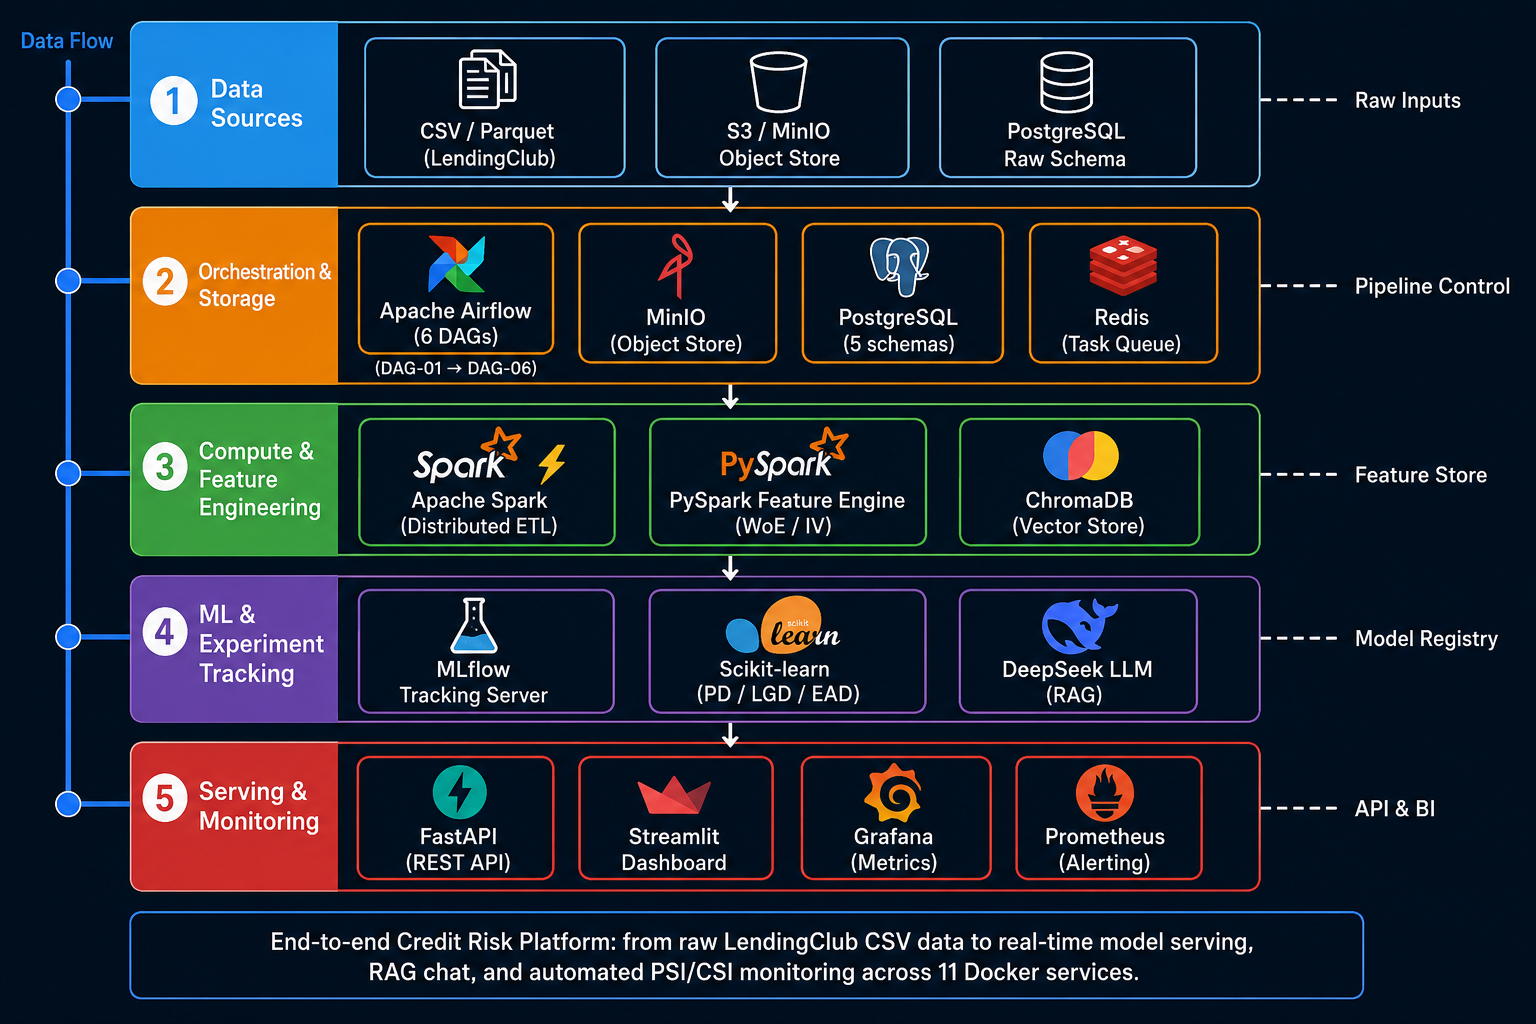
\includegraphics[width=\textwidth]{system_architecture.png}
\caption{Five-layer credit risk system architecture overview}
\label{fig:sysarch}
\end{figure}

\medskip
\noindent The diagram reveals a clean separation of concerns across the five layers. Data flows strictly downward: raw records enter through MinIO, progress through the orchestration and processing layers, and exit as scored outputs and regulatory reports through the risk layer. This unidirectional dependency structure means any upstream component can be modified or replaced without affecting downstream consumers, provided the artefact contracts (table schemas and file formats) are maintained.

\section{Technology Stack}

% ─────────────────────────────────────────────────────────────────────────────
% IMAGE GENERATION PROMPT — tech_stack.png
% Place the generated image in: docs/images/tech_stack.png
%
% PROMPT:
% Create a clean, professional infographic titled "Technology Stack — Credit Risk
% Data Engineering Pipeline" for use in an academic report.
%
% Layout: a vertical stack of 5 horizontal bands, each band representing one
% system layer. Left of each band: a solid colour label box (dark navy
% #003366) containing the layer name in white bold text. Right: an icon-and-
% text cell for each technology in that layer.
%
% Bands (top to bottom):
%   1. ORCHESTRATION — Apache Airflow 2.x (dag icon, scheduler icon)
%   2. BIG DATA / PROCESSING — Apache Spark 3.x + PySpark (lightning bolt), MinIO (bucket)
%   3. DATA WAREHOUSE — PostgreSQL 15 (elephant logo style), Great Expectations (shield)
%   4. ML / SERVING — MLflow (flask icon), Statsmodels, Scikit-learn, FastAPI + Redis
%   5. MONITORING — Prometheus (fire icon), Grafana (bar chart), Docker Compose (whale)
%
% Each technology cell shows: a small representative icon + technology name +
% one-line purpose in grey italic (e.g. "DAG scheduling & audit trail").
%
% Colour scheme: navy blue (#003366) labels, white card backgrounds, light
% grey (#F5F5F5) alternating band background, gold (#B47800) accent borders.
% Corporate, minimal, no shadows, no gradients. Font: sans-serif, clean.
% Output size: 1600 × 900 px PNG, white background.
% ─────────────────────────────────────────────────────────────────────────────

The following figure summarises the technology choices and rationale for each system layer. The stack is selected to balance regulatory auditability (statsmodels, MLflow governance gates), performance (PySpark column projection, Redis caching), and reproducibility (Docker Compose single-command deployment).

\begin{figure}[H]
\centering
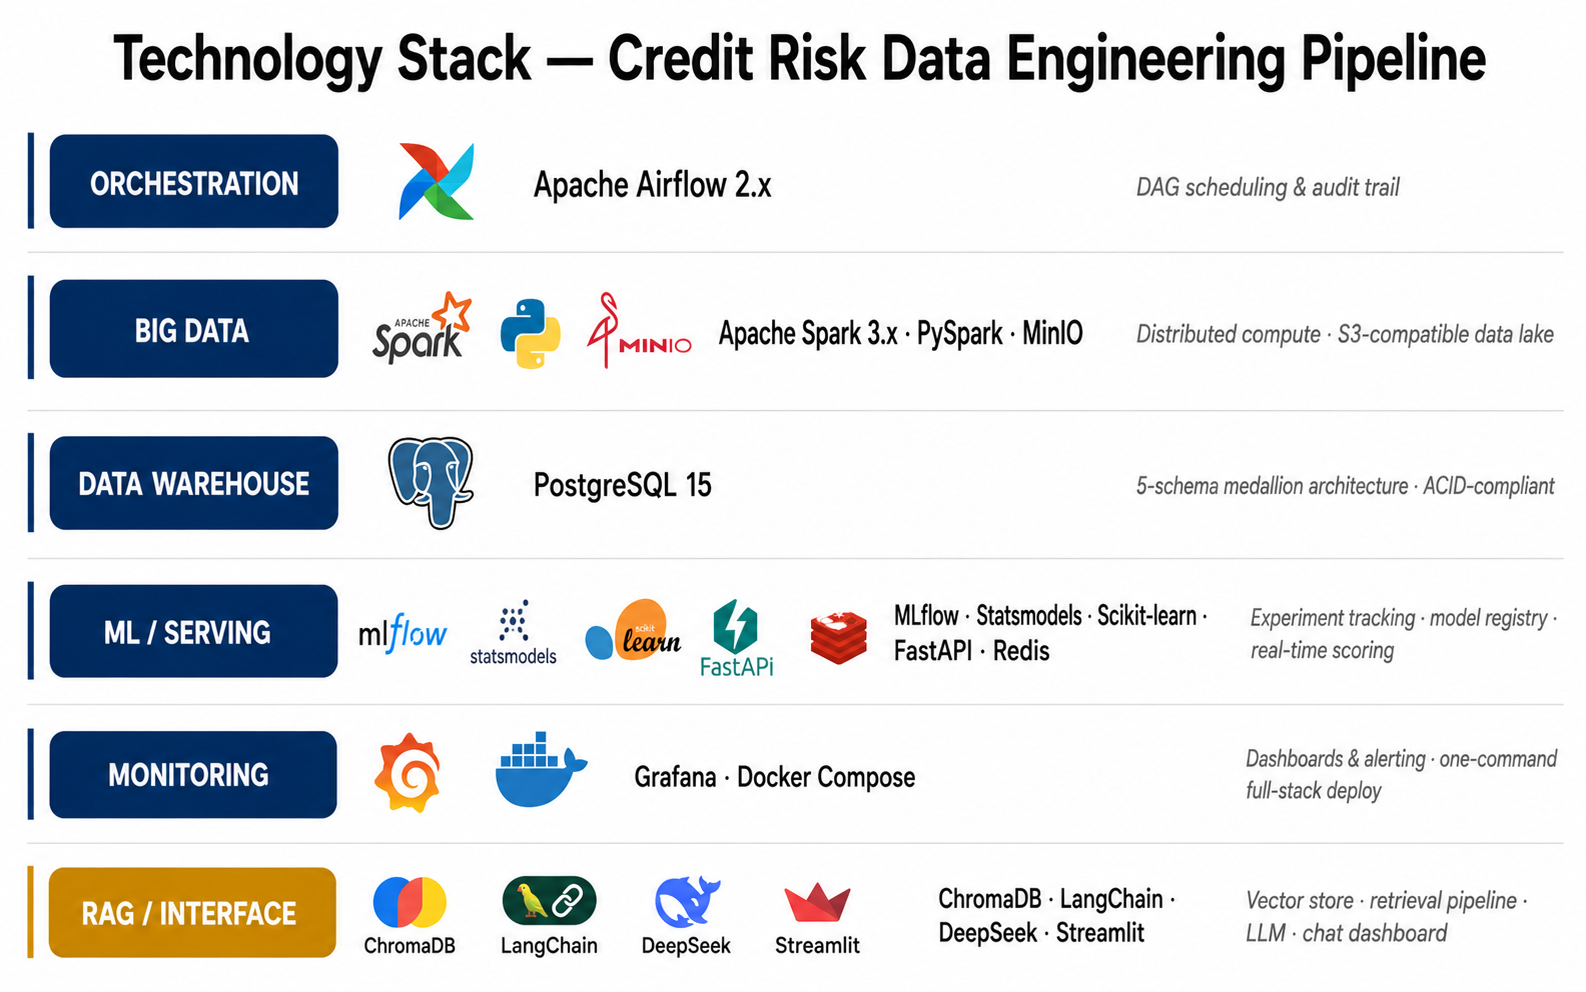
\includegraphics[width=\textwidth]{tech_stack.png}
\caption{Technology stack and rationale for each pipeline layer}
\label{fig:techstack}
\end{figure}

\medskip
\noindent The layered technology selection reflects a key principle: no single tool handles all concerns. Airflow owns scheduling and dependency management; Spark owns data volume; PostgreSQL owns ACID compliance and auditability; MLflow owns model governance; and Prometheus/Grafana own observability. Each tool is industry-standard in its domain, reducing operational risk from niche tooling choices.

\section{End-to-End Data Flow}

% ─────────────────────────────────────────────────────────────────────────────
% IMAGE GENERATION PROMPT — data_flow.png
% Place the generated image in: docs/images/data_flow.png
%
% PROMPT:
% Create a professional data flow diagram for a credit risk data engineering
% pipeline, suitable for an academic report. Style: clean flowchart on white
% background, left-to-right or top-to-bottom layout.
%
% Nodes (rectangular with rounded corners):
%   SOURCE: "accepted_2007_to_2018Q4.csv" (151 cols, 2.26M rows) — light grey
%
%   DAG-01 INGESTION (navy blue):
%     PySpark column-projected read (26/151 cols) →
%     Output: [MinIO: s3a://landing-zone/raw/] + [PostgreSQL: raw.loan_applications]
%
%   DAG-02 CLEANING (steel blue):
%     57 columns dropped | 3 targets created | OOT split flagged →
%     Output: [MinIO: s3a://spark-output/staging/] + [PostgreSQL: staging.loans_cleaned (94 cols)]
%
%   DAG-02b FEATURE ENGINEERING (teal):
%     WoE bins fitted on TRAIN only | 56 dummy variables →
%     Output: [PostgreSQL: features.woe_bins] + [features.loan_features_encoded]
%
%   FORK: two parallel branches below DAG-02b
%
%   DAG-03 PD TRAINING (amber/gold):
%     Logistic regression | p-value selection | PDO scaling | Calibration →
%     Output: [MLflow: PD-Scorecard] + [scorecard.csv] + [pd_calibrator.json]
%
%   DAG-04 LGD/EAD TRAINING (amber/gold):
%     Stage1 LogReg | Stage2 LinearReg | EAD LinearReg →
%     Output: [MLflow: LGD-Stage1/2] + [lgd_stage1.pkl] + [ead_model.pkl]
%
%   MERGE: DAG-03 + DAG-04 → DAG-05
%
%   DAG-05 BATCH SCORING (dark green):
%     EL = PD × LGD × EAD | IFRS9 ECL | Basel III AIRB →
%     Output: [risk.expected_loss] + [risk.ifrs9_provisions] + [risk.capital_requirements]
%
%   DAG-06 MONITORING (red-orange):
%     PSI / CSI daily | Champion-Challenger | Vintage analysis →
%     Output: [Prometheus metrics] + [Grafana alerts]
%
% Arrows: solid dark grey with arrowheads. Label each arrow with the key
% artefact being passed (e.g. "Parquet + JDBC"). Show the parallel fork and
% merge clearly with a horizontal split-merge junction.
%
% Footer note: "All DAGs orchestrated by Apache Airflow. Full run time: ~3 min."
% Output size: 1800 × 1100 px PNG, white background, corporate sans-serif font.
% ─────────────────────────────────────────────────────────────────────────────

Figure~\ref{fig:dataflow} illustrates the end-to-end data flow through all six pipeline DAGs, from raw CSV ingestion through to daily monitoring outputs.

\begin{figure}[H]
\centering
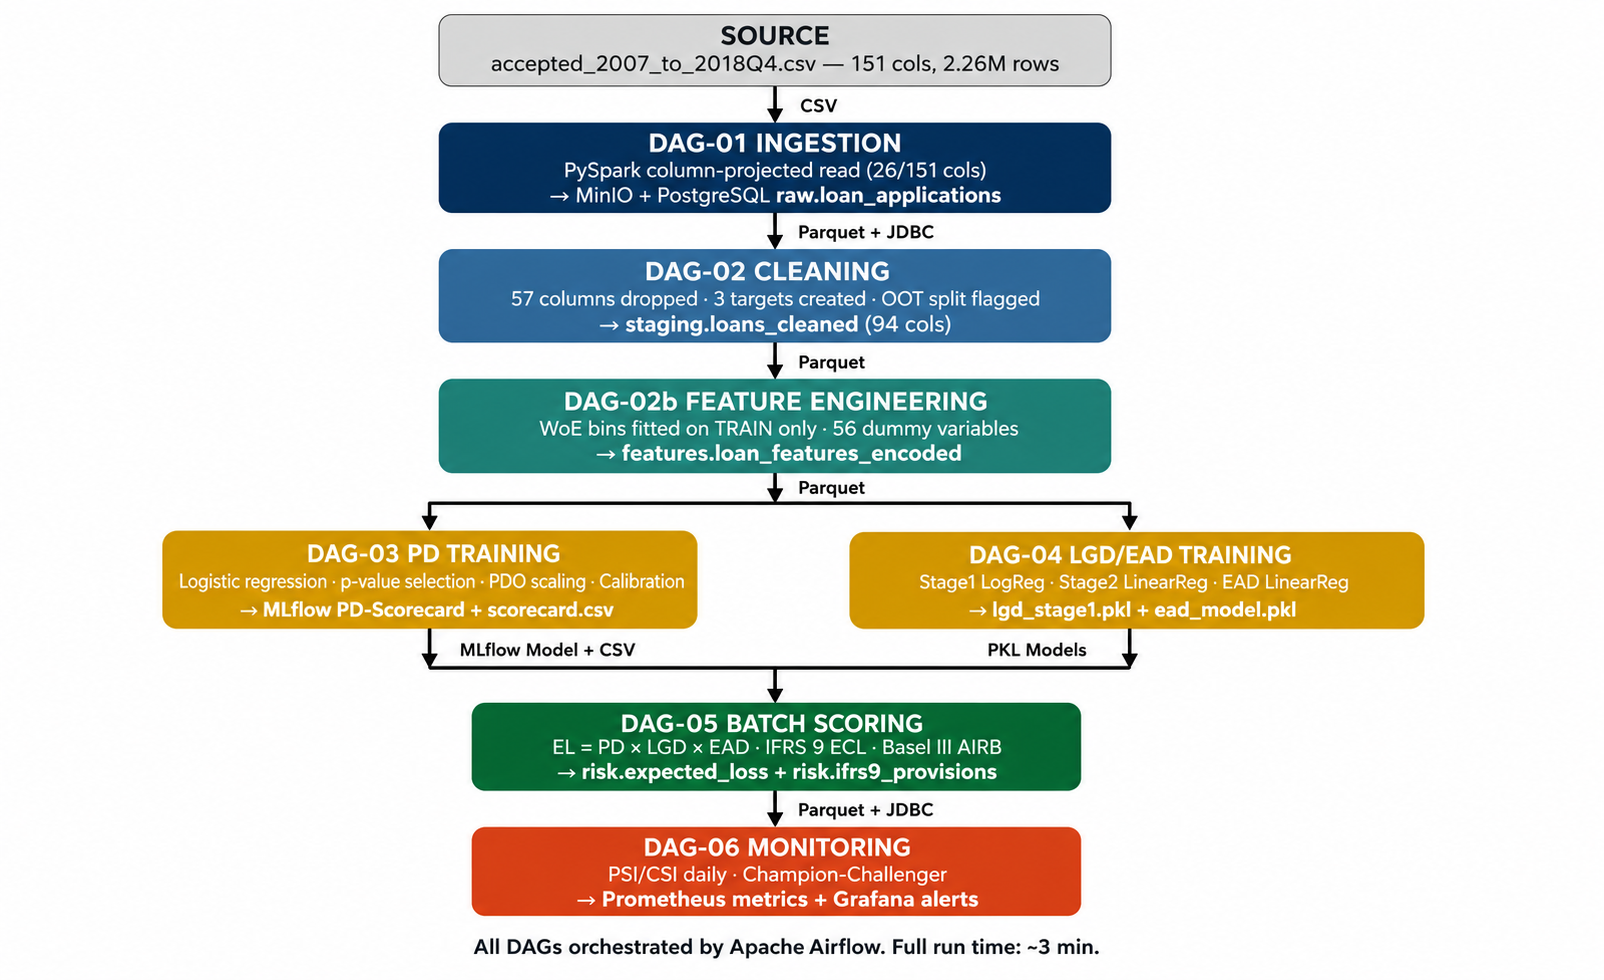
\includegraphics[width=\textwidth]{data_flow.png}
\caption{End-to-end data flow through the six pipeline DAGs}
\label{fig:dataflow}
\end{figure}

\medskip
\noindent The fork-and-merge pattern between DAG-02b and DAG-05 is a critical design feature: by running the PD and LGD/EAD training pipelines in parallel, total model rebuild time is reduced. Both branches read from the same WoE-encoded feature store but write to separate MLflow experiment namespaces, ensuring their artefacts are independently versioned and auditable.

\section{Infrastructure: Docker Compose Services}

The full stack runs as 11 Docker Compose services:

\begin{lstlisting}[language=bash, caption={Key Docker Compose services}]
services:
  postgres:          # Data warehouse (5 schemas)
  minio:             # Data lake (S3-compatible)
  spark-master:      # Spark coordinator node
  spark-worker:      # Spark executor node
  airflow-webserver: # Airflow UI and API
  airflow-scheduler: # DAG scheduling engine
  mlflow:            # Experiment tracking + model registry
  api:               # FastAPI scoring service
  redis:             # Feature cache for real-time scoring
  prometheus:        # Metrics collection
  grafana:           # Dashboards and alerting
\end{lstlisting}

\medskip
\noindent The service list reflects the principle of one concern per container. The Spark master and worker are separated to allow horizontal scaling in a real cluster deployment: adding spark-worker replicas requires only a single line change in the Compose file. The entire stack starts with a single command: \texttt{make up} (which wraps \texttt{docker compose up --build -d}). All service-to-service communication uses Docker internal networking; no port is exposed to the public internet by default.

\section{Streamlit Monitoring Dashboard}

A Streamlit dashboard (\texttt{dashboard.py}) provides a browser-based interface to the pipeline outputs, integrating the credit risk monitoring charts, the IFRS~9 and Basel~III regulatory outputs, and the RAG chat interface into a single application.

\begin{figure}[H]
\centering
\fbox{\parbox{0.88\textwidth}{\centering\vspace{2.5cm}
{\large\textbf{[Screenshot Placeholder: Streamlit Monitoring Dashboard]}}\\[0.6cm]
\textit{Replace with a screenshot of the Streamlit dashboard showing the Credit Risk Portfolio\\
page with KPI cards (Total EAD, EL Rate, IFRS~9 Stage distribution) and sidebar navigation.}\\[0.4cm]
\textbf{File name:} \texttt{dashboard\_screenshot.png} \quad
\textbf{Suggested size:} 1600$\times$900\,px PNG
\vspace{2.5cm}}}
\caption{Streamlit credit risk monitoring dashboard (screenshot placeholder)}
\label{fig:dashboard}
\end{figure}

\medskip
\noindent The dashboard is launched via \texttt{streamlit run dashboard.py} and is accessible at \texttt{http://localhost:8501}. It connects to the PostgreSQL risk schema and the ChromaDB vector stores, so all panels display live data from the most recent pipeline run. The sidebar navigation separates monitoring views from the RAG chat interface, allowing technical and non-technical users to work in the same tool without confusion.

% ─────────────────────────────────────────────────────────────────────────────
\chapter{Database Design}
\label{ch:db}
% ─────────────────────────────────────────────────────────────────────────────

\section{Five-Schema Medallion Architecture}

The PostgreSQL data warehouse implements a medallion architecture with five logical schemas, each representing a distinct stage of data maturity.

\begin{figure}[H]
\centering
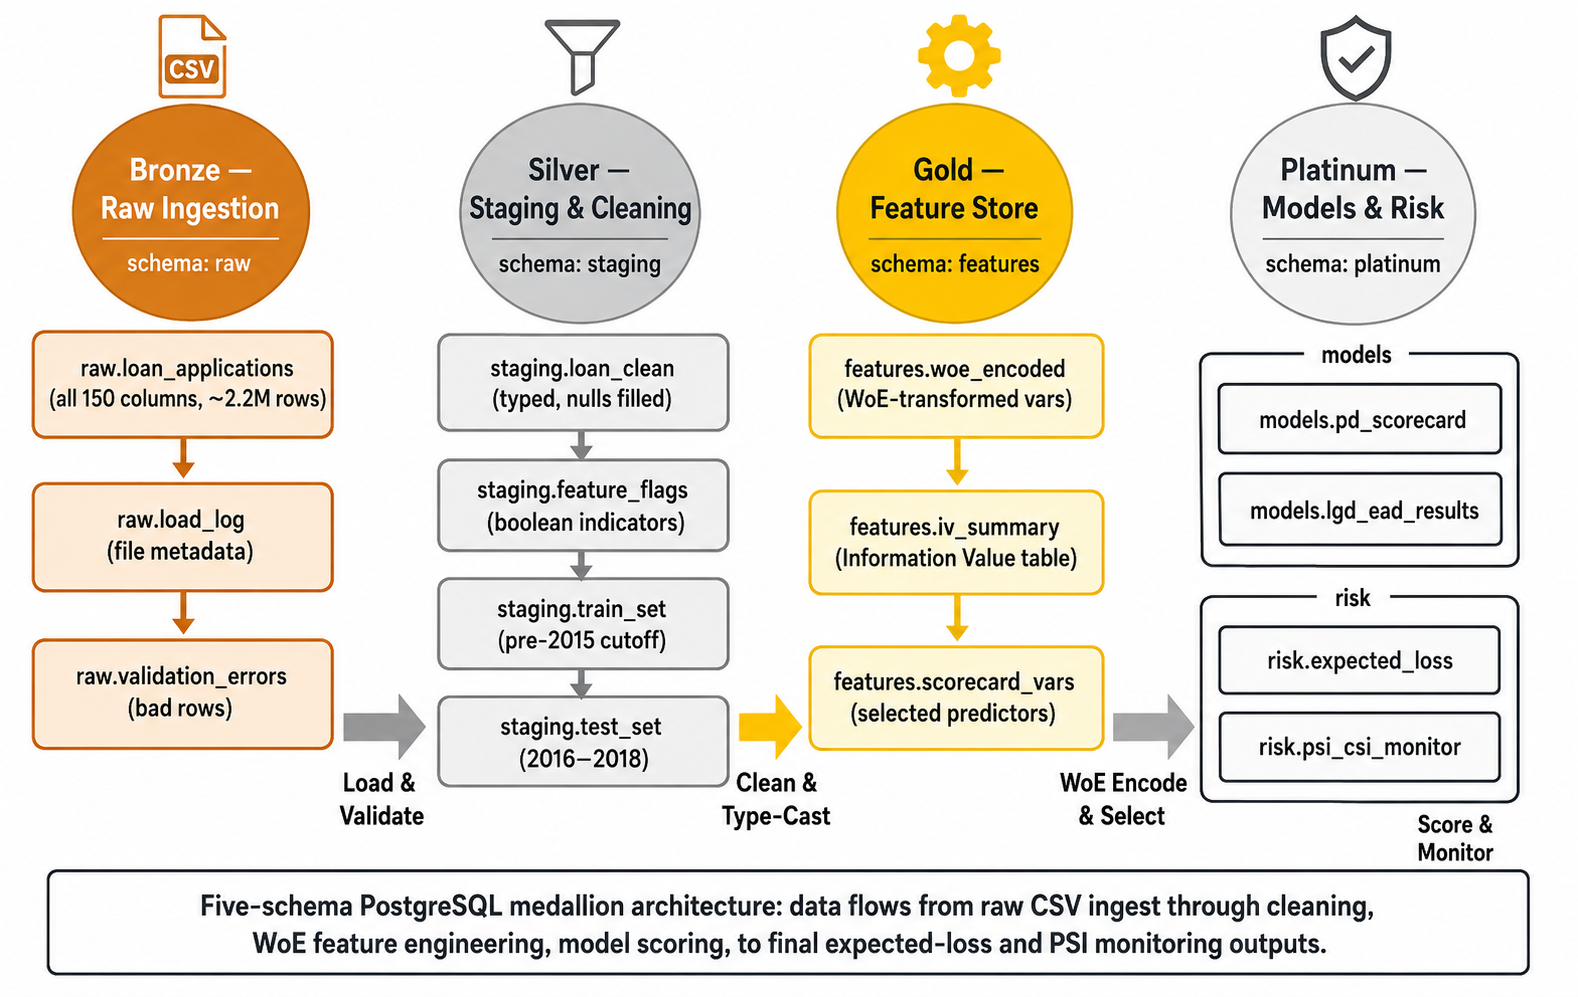
\includegraphics[width=\textwidth]{medallion_architecture.png}
\caption{PostgreSQL medallion architecture: Bronze (raw) $\to$ Silver (staging) $\to$ Gold (features, models, risk)}
\label{fig:medallion}
\end{figure}

\medskip
\noindent The medallion architecture enforces data quality discipline through physical schema separation rather than access controls alone. Data in the raw schema is append-only and immutable; transformations always produce new rows in the downstream schema rather than updating existing ones. This insert-only pattern creates a natural audit trail: any intermediate state of the pipeline can be reconstructed by re-running the appropriate DAG starting from the raw schema, without touching the source data.

\begin{table}[H]
\centering
\caption{PostgreSQL schema design}
\label{tab:schemas}
\begin{tabularx}{\textwidth}{llX}
\toprule
\textbf{Schema} & \textbf{Layer} & \textbf{Purpose and Key Tables} \\
\midrule
\texttt{raw}      & Bronze & Untouched CSV data loaded as-is from MinIO. \texttt{loan\_applications} (151 cols, 2.26M rows). No transformations; append-only. \\
\texttt{staging}  & Silver & Cleaned, type-corrected, validated data. \texttt{loans\_cleaned} (94 cols) with OOT split flag (\texttt{dataset\_split = 'train' | 'oot'}). Target variables created here. \\
\texttt{features} & Gold   & WoE bins, dummy variables, information values. \texttt{woe\_bins} (fitted on training set only). \texttt{loan\_features\_encoded} (56 WoE dummies). \texttt{information\_values} per feature. \\
\texttt{models}   & Gold   & Model predictions and scores. \texttt{pd\_scores} (credit score, PD, risk class). \texttt{lgd\_ead\_scores} (LGD, EAD per loan). \\
\texttt{risk}     & Gold   & Business risk outputs and regulatory reports. \texttt{expected\_loss}, \texttt{ifrs9\_provisions}, \texttt{capital\_requirements}, \texttt{population\_stability}, \texttt{credit\_policy\_decisions}. \\
\bottomrule
\end{tabularx}
\end{table}

\medskip
\noindent The five-schema design reflects a strict layering principle: each schema reads only from schemas to its left and writes only to itself. The raw schema is populated by the ingest DAG; staging by cleaning; features by feature engineering; and models and risk by training and scoring DAGs respectively. This unidirectional dependency prevents circular data flows and ensures each schema's contents can always be regenerated from its upstream schema without loss of information.

\section{Key Design Decisions}

\textbf{Out-of-time split flag in staging.} The \texttt{dataset\_split} column (\texttt{'train'} for 2007--2015, \texttt{'oot'} for 2016--2018) is set during the cleaning DAG and propagates through all downstream schemas. This ensures that WoE bins are always fitted exclusively on training-set rows and that OOT data is never used to fit any model parameters --- a critical discipline for preventing look-ahead bias.

\textbf{WoE bins stored separately from encoded features.} The \texttt{features.woe\_bins} table stores the bin boundaries and WoE values computed on the training set. The \texttt{features.loan\_features\_encoded} table stores the resulting binary dummy columns. This separation means the WoE mapping can be versioned, audited, and applied to new data independently of any model retraining.

\textbf{Per-loan IFRS~9 records with audit fields.} The \texttt{risk.ifrs9\_provisions} table stores the IFRS~9 stage (1, 2, or 3), the SICR trigger reason, the 12-month ECL, the lifetime ECL under each macroeconomic scenario, and the probability-weighted ECL. Every record carries a \texttt{model\_run\_id} and \texttt{calc\_date} for full audit traceability.

% ─────────────────────────────────────────────────────────────────────────────
\chapter{The Six Pipeline DAGs}
\label{ch:pipelines}
% ─────────────────────────────────────────────────────────────────────────────

The system contains six Apache Airflow DAGs, each responsible for a distinct pipeline stage. Figure~\ref{fig:dag_chain} shows the DAG dependency as a visual pipeline diagram.

\begin{figure}[H]
\centering
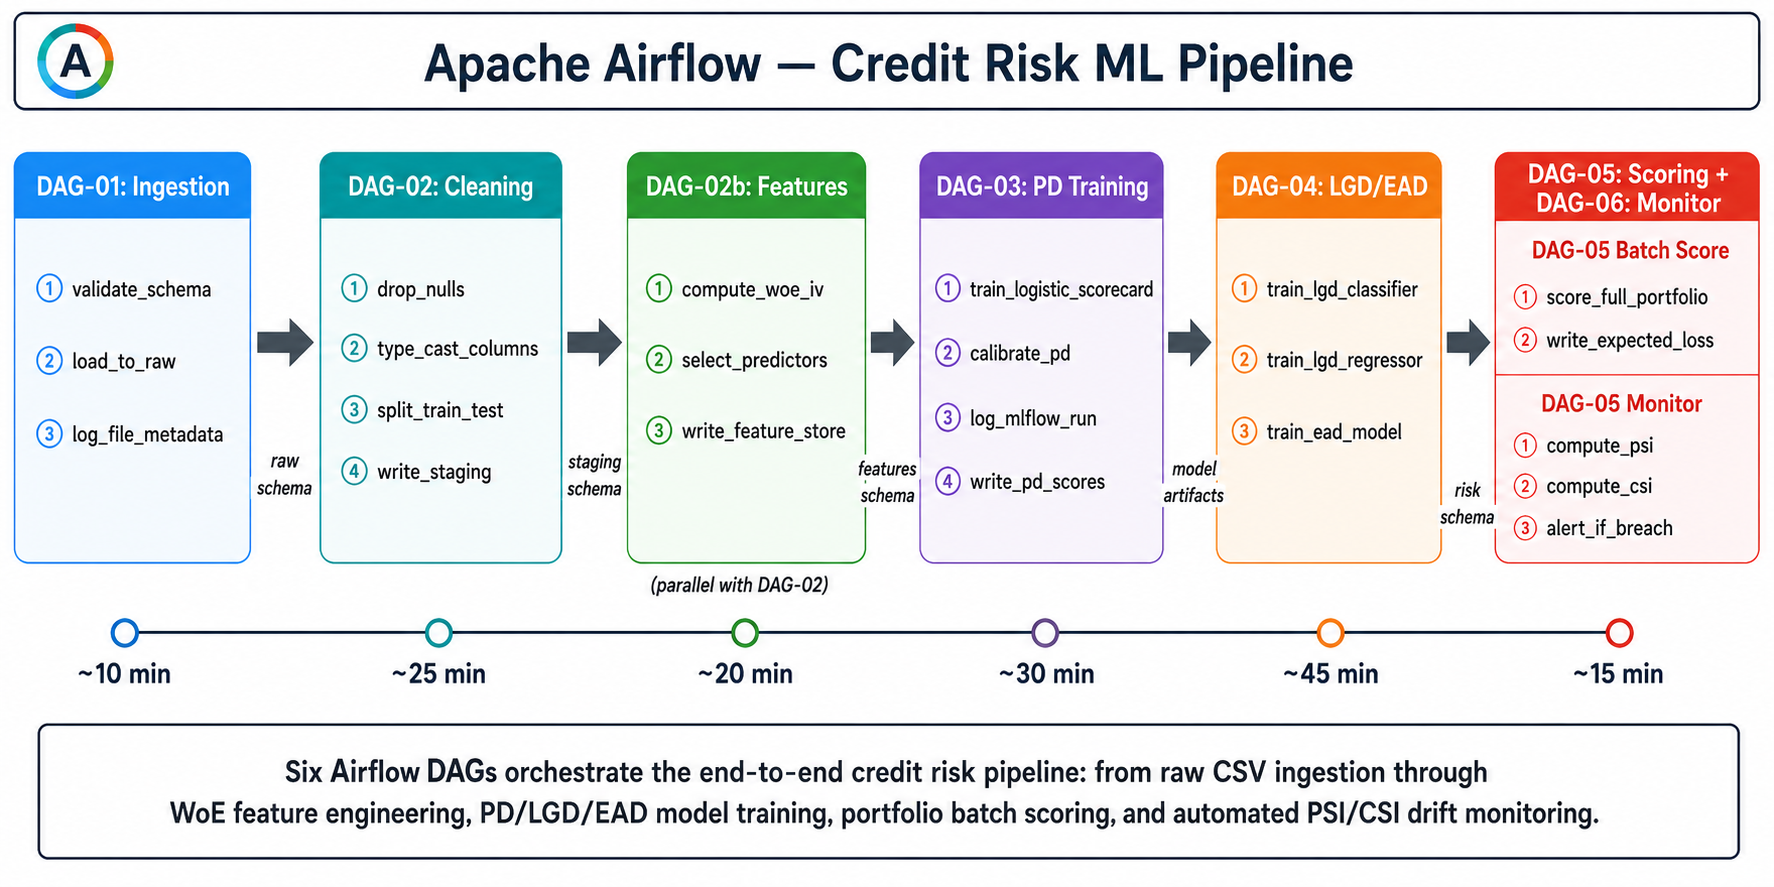
\includegraphics[width=\textwidth]{dag_pipeline.png}
\caption{Airflow DAG dependency chain --- from ingestion to monitoring}
\label{fig:dag_chain}
\end{figure}

\medskip
\noindent The DAG dependency structure reveals two key design properties. First, the pipeline is partially parallelisable: DAG-03 (PD training) and DAG-04 (LGD/EAD training) run concurrently once DAG-02b completes, reducing total wall-clock time for a full model rebuild. Second, DAG-06 (monitoring) is connected to DAG-05 but also runs on an independent daily schedule, ensuring that model health is monitored even when no new model training occurs.

% ─────────────────────────────────────────────────────────────────────────────
% IMAGE GENERATION PROMPT — dag_dependency.png
% Place the generated image in: docs/images/dag_dependency.png
%
% PROMPT:
% Create a clean DAG dependency diagram for an Apache Airflow-based credit risk
% pipeline. Style: swimlane or top-down node-edge graph on white background.
%
% Nodes (rounded rectangles, navy blue #003366 fill, white text):
%   DAG-01: Data Ingestion
%   DAG-02: Data Cleaning
%   DAG-02b: Feature Engineering (WoE)
%   DAG-03: PD Model Training       [in GOLD #B47800]
%   DAG-04: LGD / EAD Training      [in GOLD #B47800]
%   DAG-05: Batch Scoring
%   DAG-06: Monitoring (daily + on-trigger)
%
% Layout (top to bottom):
%   DAG-01
%     ↓
%   DAG-02
%     ↓
%   DAG-02b
%   ↙        ↘
% DAG-03    DAG-04
%   ↘        ↙
%   DAG-05
%     ↓
%   DAG-06
%
% Show a dashed grey self-loop arrow on DAG-06 labelled "also runs daily @ 06:00"
% to indicate independent scheduling.
%
% Label each arrow with a short artefact name:
%   DAG-01 → DAG-02: "raw.loan_applications"
%   DAG-02 → DAG-02b: "staging.loans_cleaned"
%   DAG-02b → DAG-03: "features.loan_features_encoded"
%   DAG-02b → DAG-04: "features.loan_features_encoded"
%   DAG-03 → DAG-05: "scorecard.csv + pd_calibrator.json"
%   DAG-04 → DAG-05: "lgd_stage1.pkl + ead_model.pkl"
%   DAG-05 → DAG-06: "risk.expected_loss + pd_scores"
%
% Below each DAG node, add a small grey italic caption:
%   DAG-01: "2.26M rows • ~7 sec"
%   DAG-02: "94 cols • OOT split"
%   DAG-02b: "56 WoE dummies"
%   DAG-03: "AUC 0.694 • Gini 0.387"
%   DAG-04: "Mean LGD 92.19%"
%   DAG-05: "EL $0.808B • RWA $14.07B"
%   DAG-06: "PSI 0.282 (ALERT)"
%
% Output size: 1200 × 1600 px PNG (portrait), white background,
% corporate sans-serif font, no drop shadows.
% ─────────────────────────────────────────────────────────────────────────────

Figure~\ref{fig:dag_dep} provides a detailed DAG dependency diagram with artefact labels on each edge, showing which specific files and tables flow between pipeline stages.

\begin{figure}[H]
\centering
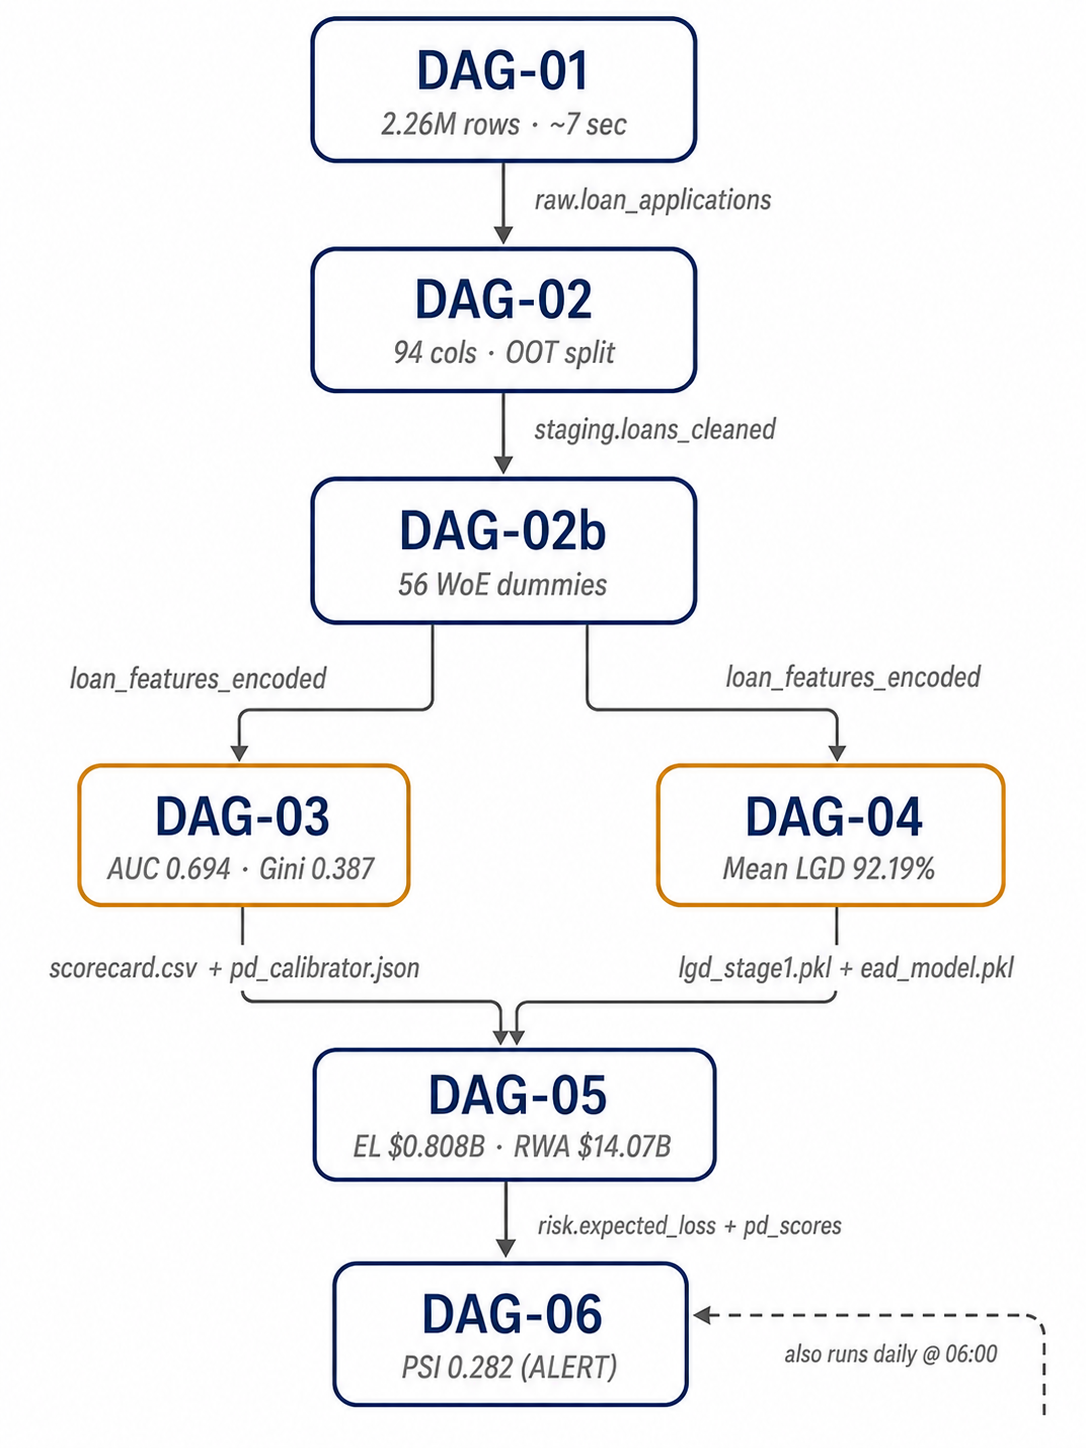
\includegraphics[width=\textwidth]{dag_dependency.png}
\caption{Airflow DAG dependency chain with artefact labels on each edge}
\label{fig:dag_dep}
\end{figure}

\section{DAG-01: Data Ingestion}

\textbf{Trigger:} Manual or scheduled when a new raw CSV is deposited in MinIO.\\
\textbf{Technology:} PySpark (column-projected read), MinIO S3A connector, PostgreSQL JDBC writer.

\textbf{What it does:}
\begin{enumerate}
  \item PySpark reads the raw \texttt{accepted\_2007\_to\_2018Q4.csv} from MinIO using \textbf{column projection} --- only the 26 modelling-relevant columns are read from the 151-column file. This reduces the Spark read time from $\approx$60 seconds (full file) to $\approx$7 seconds and mirrors real ETL practice: columns that are immediately dropped should never be loaded into memory.
  \item Basic type casting is applied at ingest time: string percentages (\texttt{int\_rate}, \texttt{revol\_util}) are converted to float; date strings (\texttt{issue\_d}, \texttt{earliest\_cr\_line}) are parsed; the \texttt{term} string (``36 months'') is converted to integer.
  \item The parsed data is written to \texttt{raw.loan\_applications} in PostgreSQL using JDBC batch write, and a backup Parquet copy is written to MinIO for Spark intermediate jobs.
\end{enumerate}

\textbf{Key engineering detail --- column projection:}
\begin{lstlisting}[language=Python, caption={Column-projected PySpark read in DAG-01}]
KEEP_COLS = [
    'funded_amnt', 'term', 'int_rate', 'grade', 'emp_length',
    'home_ownership', 'annual_inc', 'verification_status', 'issue_d',
    'loan_status', 'purpose', 'dti', 'earliest_cr_line',
    'fico_range_low', 'fico_range_high', 'inq_last_6mths',
    'mths_since_last_delinq', 'revol_util', 'initial_list_status',
    'pct_tl_nvr_dlq', 'total_pymnt', 'recoveries', 'funded_amnt',
    'out_prncp', 'last_pymnt_d', 'mths_since_last_record'
]

df = (spark.read
    .option("header", "true")
    .option("inferSchema", "true")
    .csv("s3a://landing-zone/raw/accepted_2007_to_2018Q4.csv")
    .select(KEEP_COLS))
\end{lstlisting}

\medskip
\noindent Column projection is the most impactful single-line performance optimisation in the pipeline. By reading only 26 of the 151 columns at the SparkSession layer, I/O volume is reduced by 83\%, which explains the 7-second versus 60-second ingest time comparison. The type corrections applied at ingest time ensure that downstream DAGs receive clean numeric types without needing to parse raw text, eliminating a common source of null-propagation errors in later transformations.

\textbf{Artefacts produced:} \texttt{raw.loan\_applications} (PostgreSQL), \texttt{s3a://spark-output/raw/*.parquet} (MinIO).

\section{DAG-02: Data Cleaning}

\textbf{Trigger:} Downstream of DAG-01 completion.\\
\textbf{Technology:} PySpark transformation job, Great Expectations validation suite.

\textbf{What it does:}
\begin{enumerate}
  \item \textbf{Column removal} --- 57 columns are removed across five categories (Table~\ref{tab:colremoval}). Post-application leakage columns (\texttt{total\_pymnt}, \texttt{recoveries}, \texttt{out\_prncp}) are used first to create the three target variables, then dropped to prevent any information from post-default events entering the feature set.
  \item \textbf{Target variable creation:}
  \begin{itemize}
    \item \texttt{good\_bad}: 1 = Fully Paid; 0 = Charged Off, Default, Late 31--120 days.
    \item \texttt{recovery\_rate}: \texttt{recoveries / funded\_amnt} on charged-off loans only (LGD target).
    \item \texttt{ccf}: \texttt{(funded\_amnt $-$ total\_pymnt) / funded\_amnt} on charged-off loans only (EAD target).
  \end{itemize}
  \item \textbf{Feature derivation:} \texttt{fico\_score} (FICO range midpoint), \texttt{term\_int}, \texttt{int\_rate} ($\div$100), \texttt{mths\_since\_issue\_d}, \texttt{mths\_since\_earliest\_cr\_line}, \texttt{emp\_length\_int}.
  \item \textbf{Out-of-time split flagging:} Each row receives \texttt{dataset\_split = 'train'} (issue year $\leq$ 2015) or \texttt{dataset\_split = 'oot'} (issue year $\geq$ 2016). Note: the raw file is NOT sorted chronologically, so the split is based on \texttt{issue\_year} derived from \texttt{issue\_d}, not on row order.
  \item \textbf{Data quality validation:} Great Expectations validates column types, null rates, and value ranges at the end of the cleaning job before writing to staging.
\end{enumerate}

\begin{table}[H]
\centering
\caption{Column removal categories in DAG-02}
\label{tab:colremoval}
\begin{tabular}{llll}
\toprule
\textbf{Category} & \textbf{Count} & \textbf{Examples} & \textbf{Reason} \\
\midrule
100\% null          & 15 & \texttt{sec\_app\_*}, \texttt{member\_id}     & No information content \\
Identifiers/constants& 8  & \texttt{id}, \texttt{url}, \texttt{policy\_code}  & Not predictive \\
Joint application   &  3  & \texttt{sec\_app\_fico\_range\_low}           & $>99\%$ null \\
Hardship/settlement & 18  & \texttt{hardship\_type}, \texttt{settlement\_*} & $>97\%$ null \\
Post-app. leakage   & 15  & \texttt{total\_pymnt}, \texttt{recoveries}   & Known only after default \\
\midrule
\textbf{Total removed} & \textbf{57} & & \\
\bottomrule
\end{tabular}
\end{table}

\medskip
\noindent The hardship and settlement columns represent the largest removal category, but their absence has no impact on predictive power: these fields were only introduced by Lending Club in later years and are empty for the majority of the dataset. The post-application leakage columns are the most dangerous category from a modelling perspective --- \texttt{total\_pymnt} and \texttt{recoveries} are knowable only after a loan has completed or defaulted, and including them as predictors would produce a model that works perfectly on historical data but cannot score any new application.

\textbf{Artefacts produced:} \texttt{staging.loans\_cleaned} (PostgreSQL, 94 columns), \texttt{s3a://spark-output/staging/*.parquet}.

\section{DAG-02b: Feature Engineering}

\textbf{Trigger:} Downstream of DAG-02 completion.\\
\textbf{Technology:} PySpark, custom WoE encoding library, PostgreSQL feature store.

This DAG performs the most domain-specific transformation in the pipeline: converting raw loan features into Weight of Evidence (WoE) encoded dummy variables suitable for logistic regression.

\textbf{Why WoE encoding?} WoE encoding provides three benefits critical in regulated banking:
(1) it handles non-linear relationships between predictors and the log-odds of default through discretisation and bin-level mapping;
(2) it treats missing values as a separate bin rather than imputing them --- missingness in credit data is often behaviourally informative;
(3) it produces monotonic partial effects that are interpretable by regulators and can be traced to individual bin assignments in SR~11-7 documentation \cite{siddiqi2006, lund2021}.

\textbf{What it does:}
\begin{enumerate}
  \item \textbf{Training-set-only fitting:} WoE bins are computed exclusively on rows where \texttt{dataset\_split = 'train'}. The fitted bin boundaries and WoE values are stored in \texttt{features.woe\_bins}.
  \item \textbf{Fine classing:} Continuous variables are first split into 10--20 quantile bins. The WoE value for each bin is computed as $WoE_i = \ln(\%Goods_i / \%Bads_i)$.
  \item \textbf{Coarse classing:} Adjacent fine bins with similar WoE values or low observation counts are merged into coarse classes to prevent overfitting and ensure monotonicity.
  \item \textbf{Dummy creation:} Each coarse class becomes a binary dummy variable. The reference category (highest-risk bin) is dropped.
  \item \textbf{OOT encoding:} The fitted bin boundaries are applied to OOT data without re-fitting.
  \item \textbf{Information Value logging:} IV for each variable is computed and stored in \texttt{features.information\_values}.
\end{enumerate}

The final feature store contains 56 WoE dummy variables derived from 16 raw predictors, written to \texttt{features.loan\_features\_encoded}.

\begin{figure}[H]
\centering
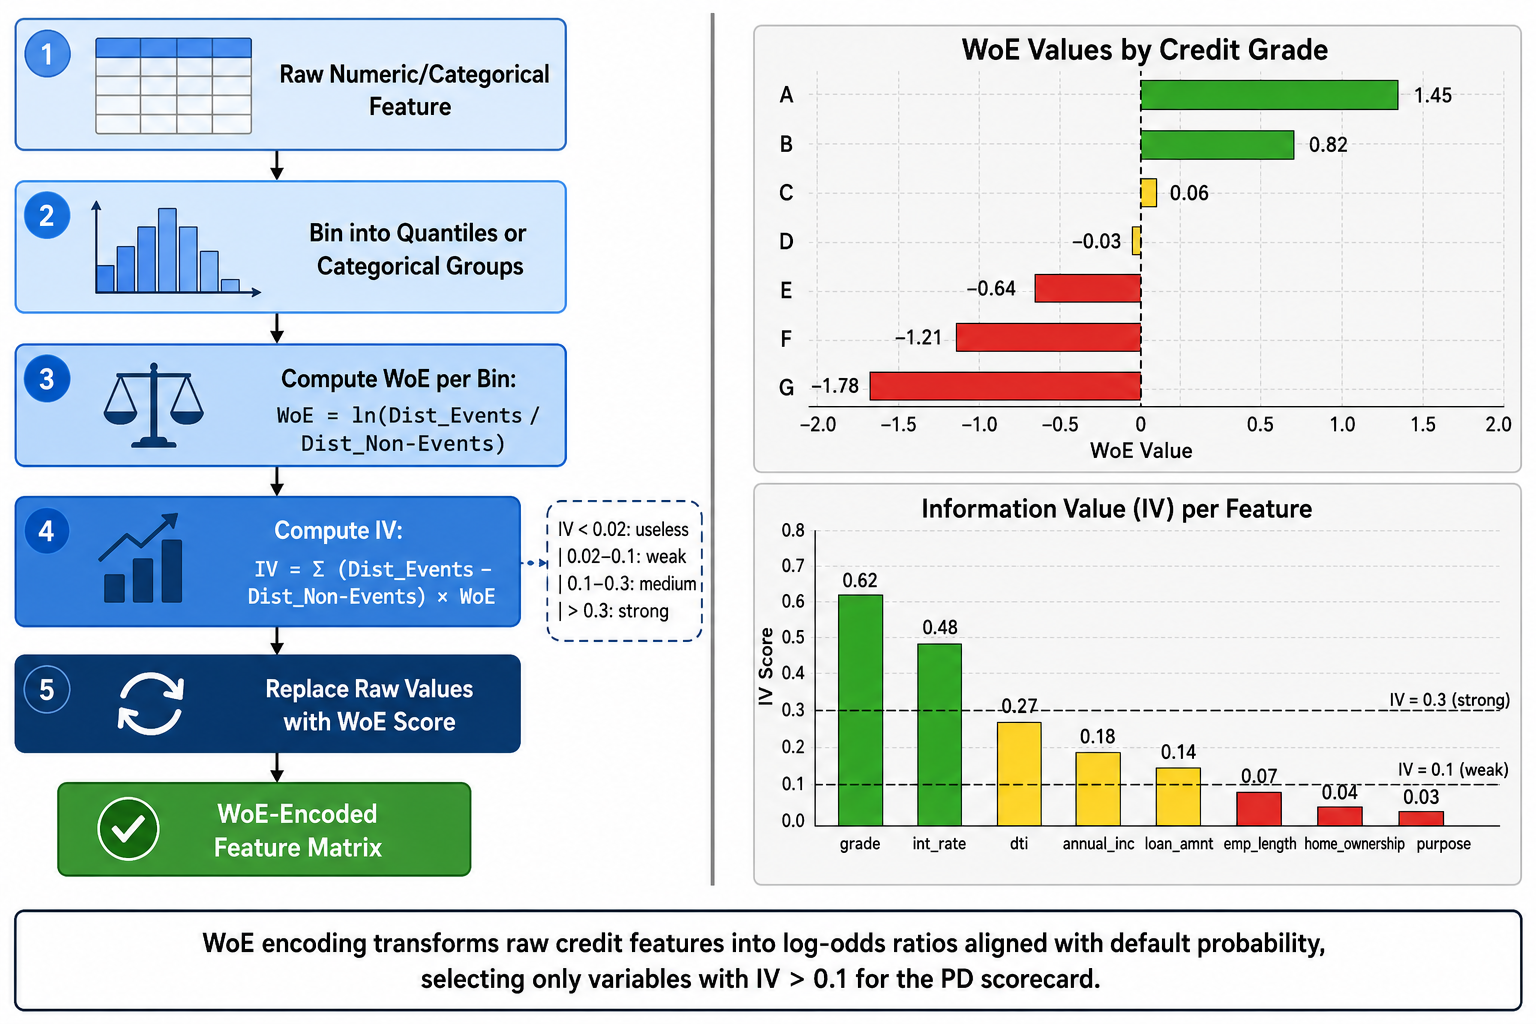
\includegraphics[width=\textwidth]{woe_encoding_flow.png}
\caption{WoE feature engineering pipeline with example Information Value (IV) per feature}
\label{fig:woe}
\end{figure}

\medskip
\noindent The Information Value chart reveals the relative predictive contribution of each feature. Variables with IV\,>\,0.3 (such as loan grade, interest rate, and FICO score) are strong predictors and receive the highest number of coarse bins. Variables with IV between 0.1 and 0.3 are medium predictors. The WoE flow ensures that all 16 raw predictors contribute to the final scorecard through at least one dummy variable, with the exact number of dummies determined by the coarse-classing step.

\textbf{Artefacts produced:} \texttt{features.woe\_bins}, \texttt{features.information\_values}, \texttt{features.loan\_features\_encoded}, \texttt{data/processed/train\_preprocessed.parquet}, \texttt{data/processed/test\_preprocessed.parquet}.

\section{DAG-03: PD Model Training}

\textbf{Trigger:} Downstream of DAG-02b. Can also be triggered independently for model re-runs.\\
\textbf{Technology:} Statsmodels (logistic regression), Scikit-learn (metrics), MLflow (tracking), Pandas.

The PD training DAG implements a full scorecard development workflow:

\begin{enumerate}
  \item \textbf{Feature selection:} Iterative backward elimination using Wald-test p-values from statsmodels. Variables with the highest maximum p-value across their dummies are removed iteratively until all remaining dummies have $p < 0.05$. This reduces the feature set from 56 to 39 statistically significant dummy variables.

  \item \textbf{Model fitting:} Logistic regression estimated with \texttt{statsmodels.Logit}. Statsmodels is used rather than scikit-learn because it provides proper Wald-test p-values and confidence intervals required for regulatory documentation under EBA/GL/2017/16 \cite{eba2017a}.

  \item \textbf{Scorecard scaling:} Coefficients are converted to integer score points using PDO scaling:
  \begin{align}
    Factor &= \frac{20}{\ln 2} \approx 28.85 \\
    Score_j &= -\lfloor \hat{\beta}_j \times Factor \rceil
  \end{align}
  The resulting scorecard maps each borrower to a 300--850 integer score where higher scores indicate lower default risk.

  \item \textbf{PD calibration:} The raw model underestimates the OOT default rate (20.18\% predicted vs 25.27\% observed). An intercept log-odds shift corrects this:
  \begin{equation}
    \hat{P}^{calib} = \sigma\!\left(\operatorname{logit}(\hat{P}^{raw}) + \delta\right), \qquad \delta = +0.3204
  \end{equation}
  The Hosmer-Lemeshow statistic drops from 10,039 to 403 after calibration (a 96\% reduction).

  \item \textbf{PiT vs TtC PD:} Two calibrated variants are saved:
  \begin{itemize}
    \item \textbf{PiT PD} (calibrated to OOT observed DR\,=\,25.27\%) --- used for IFRS~9 ECL.
    \item \textbf{TtC PD} (shifted to long-run DR\,=\,15\%) --- used for Basel~III AIRB capital.
  \end{itemize}

  \item \textbf{MLflow logging:} All hyperparameters, metrics (AUC, Gini, KS, Brier, Hosmer-Lemeshow), and artefacts (scorecard CSV, calibrator JSON, PD prediction arrays) are logged to MLflow under the \texttt{PD-Scorecard} experiment.

  \item \textbf{Reject inference:} The parceling method adds 26,129 synthetic rejected-applicant rows to the training set, partially correcting the selection bias from training exclusively on funded (accepted) loans.
\end{enumerate}

\textbf{MLflow model promotion workflow:} The trained model is registered in the MLflow model registry as version \texttt{Staging}. Promotion to \texttt{Production} requires passing all governance checkpoints (AUC\,>\,0.65, monotonic decile ordering confirmed, Brier\,$\leq$\,0.20) and explicit approval from the model owner.

\begin{figure}[H]
\centering
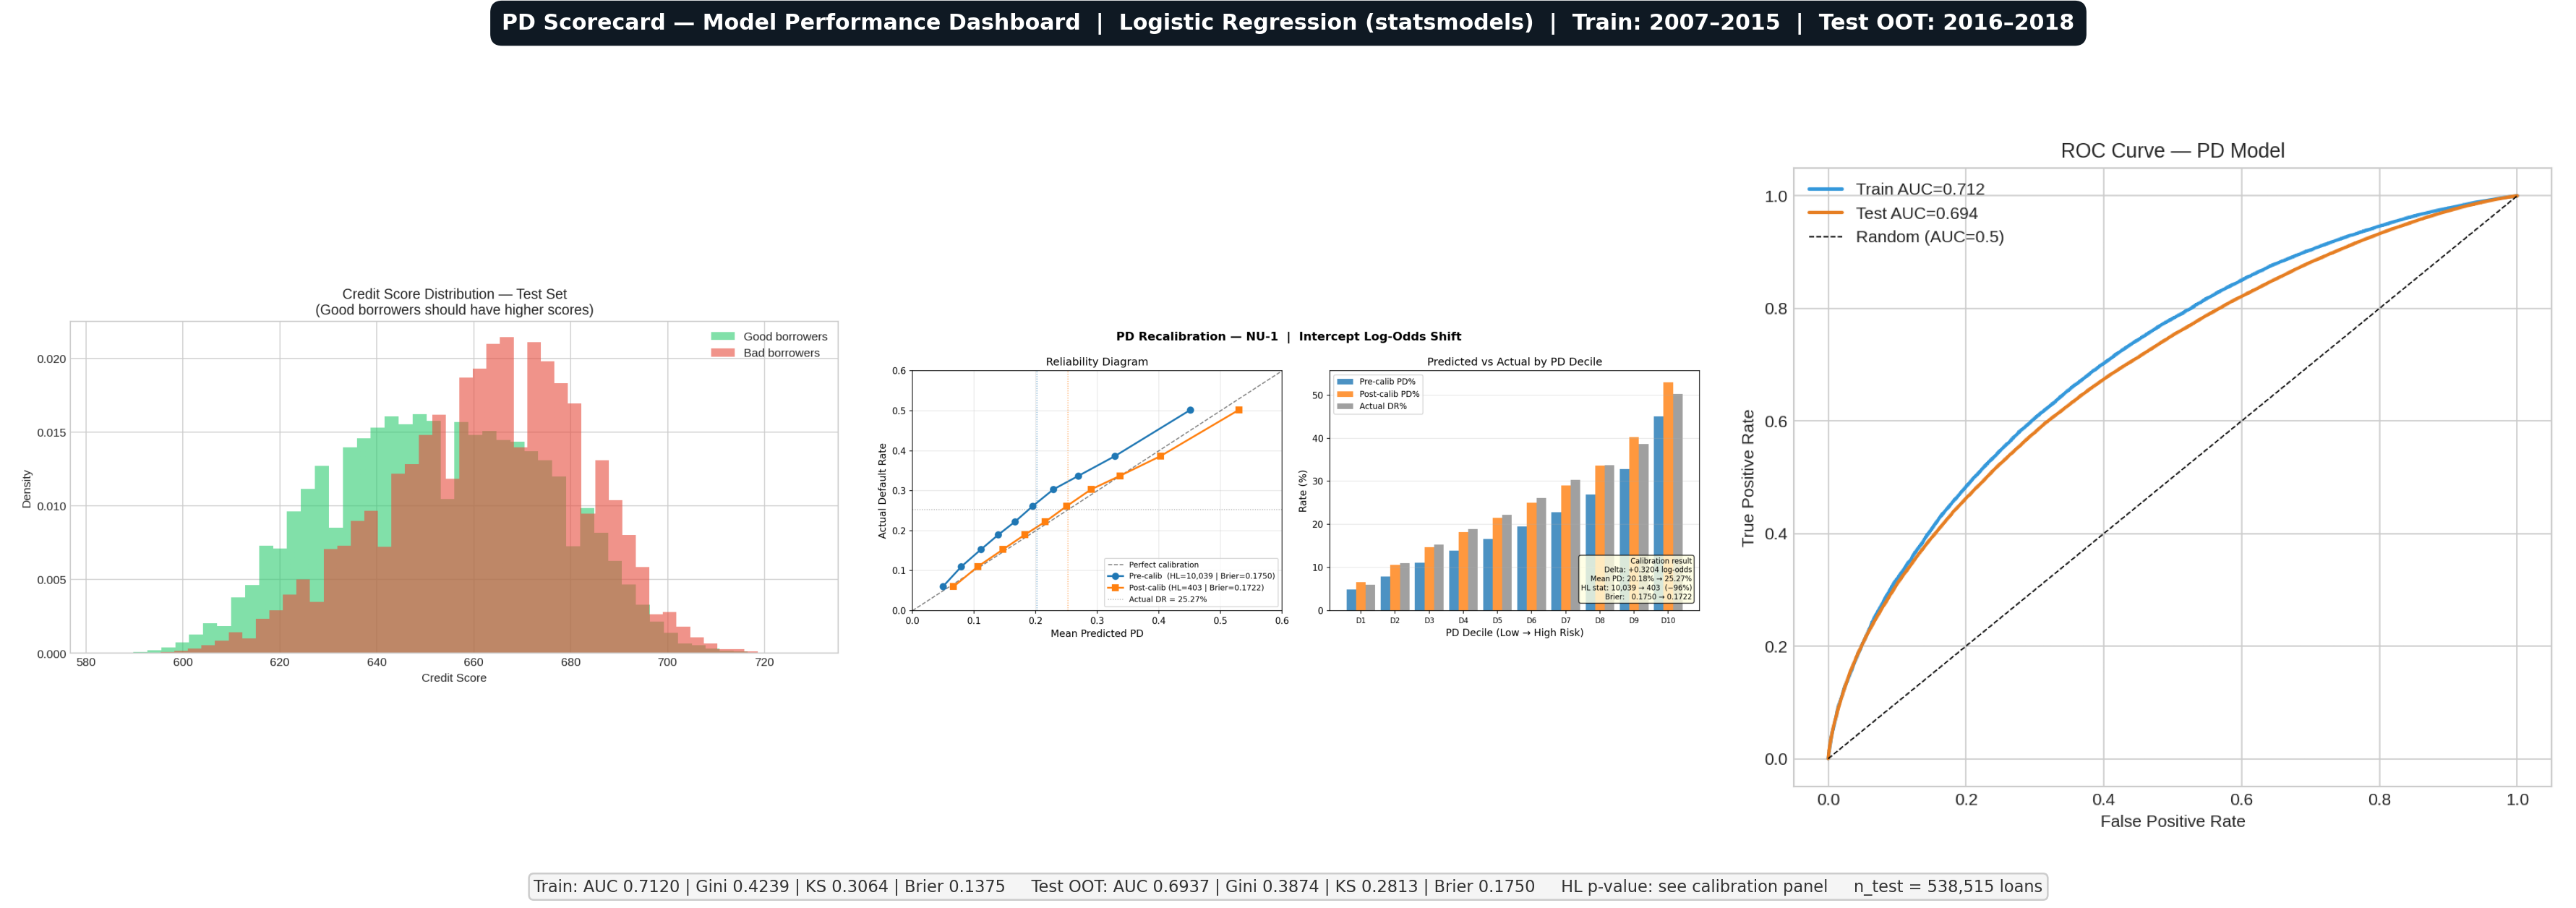
\includegraphics[width=\textwidth]{pd_scorecard_performance.png}
\caption{PD model performance: score distribution by outcome, PD calibration (pre/post), and ROC curve (AUC\,=\,0.694, Gini\,=\,0.387, OOT)}
\label{fig:pd_perf}
\end{figure}

\medskip
\noindent The three panels together tell a coherent model quality story. The score distribution shows good separation between defaulted and good loans, with the defaulted population concentrated at lower scores. The calibration reliability diagram shows the post-calibration curve closely tracking the 45-degree perfect-calibration line, confirming that the intercept shift corrects the systematic under-prediction of the raw model. The ROC curve with AUC\,=\,0.694 (Gini\,=\,0.387) on the out-of-time test set exceeds the minimum regulatory threshold of AUC\,=\,0.65, indicating acceptable discriminatory power for regulatory purposes.

\textbf{Artefacts produced:} \texttt{data/processed/scorecard.csv}, \texttt{data/models/pd\_calibrator.json}, \texttt{data/processed/pd\_pred\_test\_pit.npy}, \texttt{data/processed/pd\_pred\_test\_ttc.npy}, \texttt{data/processed/pd\_pred\_test\_pit\_calibrated.npy}, MLflow run logs.

\section{DAG-04: LGD and EAD Model Training}

\textbf{Trigger:} Downstream of DAG-02b (runs in parallel with DAG-03).\\
\textbf{Technology:} Scikit-learn (LogisticRegression, LinearRegression, StandardScaler), MLflow.

\textbf{LGD two-stage architecture:} The LGD model is applied only to charged-off loans. The bimodal distribution of recovery rates --- approximately 50.2\% of defaulted loans show zero recovery and 49.8\% show positive recovery rates --- motivates a two-stage design:
\begin{itemize}
  \item \textbf{Stage~1 (Logistic Regression):} $P(\text{Recovery Rate} > 0)$ --- predicts whether any recovery occurs.
  \item \textbf{Stage~2 (Linear Regression):} $E[\text{Recovery Rate} \mid \text{Recovery Rate} > 0]$ --- predicts the recovery amount given recovery occurs.
  \item \textbf{Combined:} $\hat{LGD} = 1 - \hat{P}_1 \times \hat{RR}_2$.
\end{itemize}

A directional constraint is enforced on the downturn LGD computation: downturn LGD must always be $\geq$ long-run LGD (recoveries fall, never rise, in a downturn). A bug in the prior implementation that violated this constraint was identified and corrected in the v4 update.

\begin{figure}[H]
\centering
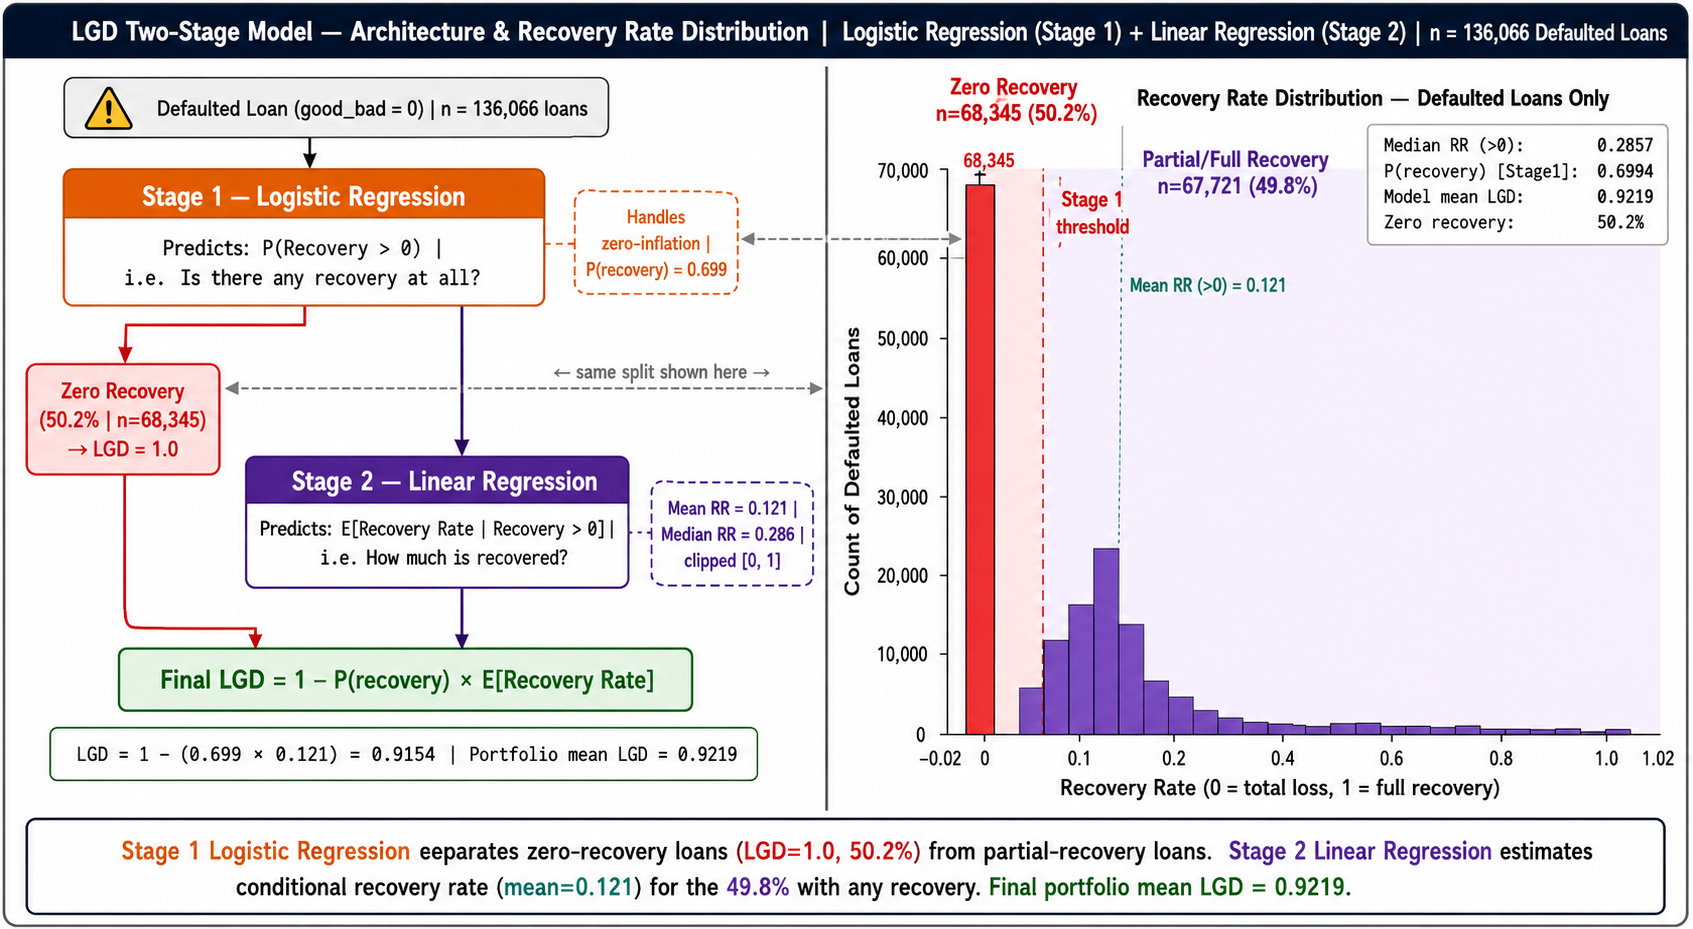
\includegraphics[width=\textwidth]{lgd_two_stage.png}
\caption{LGD two-stage model: bimodal recovery rate distribution and two-stage regression architecture}
\label{fig:lgd}
\end{figure}

\medskip
\noindent The bimodal distribution in the left panel is the empirical justification for the two-stage architecture. With 50.2\% of defaulted loans showing zero recovery, a single regression model would systematically under-predict the zero-recovery cases. The two-stage design separates the zero/non-zero decision (Stage~1, logistic) from the recovery amount prediction (Stage~2, linear), allowing each sub-model to be evaluated independently. The verified mean LGD of 92.19\% is consistent with typical unsecured consumer lending recovery rates in the academic literature.

\textbf{EAD model:} Linear regression on the Credit Conversion Factor (CCF\,$=$\,outstanding balance fraction at default). EAD\,$=$\,CCF\,$\times$\,funded\_amnt. Predictions are clipped to $[0, 1]$.

\textbf{Artefacts produced:} \texttt{data/models/lgd\_stage1.pkl}, \texttt{data/models/lgd\_stage2.pkl}, \texttt{data/models/ead\_model.pkl}, \texttt{data/models/ead\_scaler.pkl}, MLflow run logs.

\section{DAG-05: Batch Scoring}

\textbf{Trigger:} Downstream of both DAG-03 and DAG-04. Runs nightly on the full OOT portfolio.\\
\textbf{Technology:} PySpark (for large-scale feature join), Scikit-learn/Statsmodels (model application), Python (risk calculations).

\textbf{What it does:}
\begin{enumerate}
  \item Loads the fitted PD, LGD, and EAD models and the WoE-encoded feature store.
  \item Applies all three models to each loan, producing per-loan PD, LGD, and EAD estimates.
  \item Computes \textbf{Expected Loss}: $EL_i = \hat{PD}_i^{PiT} \times \hat{LGD}_i \times \hat{EAD}_i$.
  \item Computes \textbf{IFRS~9 ECL} for each loan: classifies into Stage 1, 2, or 3; computes 12-month ECL for Stage~1 and lifetime ECL (geometric hazard) for Stages~2 and~3; applies three-scenario probability-weighted ECL.
  \item Computes \textbf{Basel~III AIRB capital}: retail IRB formula with 99.9\% worst-case PD, downturn LGD, and $RWA = 12.5 \times K \times EAD$.
  \item Determines the \textbf{credit policy decision} and generates ECOA Regulation~B adverse action codes for rejections.
\end{enumerate}

\textbf{A critical v4 correction:} Prior versions used hard-coded grade-to-PD proxy tables instead of the real scorecard PD predictions. The v4 update connected the batch scoring DAG to the \texttt{pd\_pred\_test\_pit\_calibrated.npy} artefact, producing a 24\% increase in computed EL (\$+158M).

\textbf{Artefacts produced:} \texttt{risk.expected\_loss}, \texttt{risk.ifrs9\_provisions}, \texttt{risk.capital\_requirements}, \texttt{risk.credit\_policy\_decisions}, \texttt{data/processed/expected\_loss\_test.parquet}.

\section{DAG-06: Model Monitoring}

\textbf{Trigger:} Daily schedule (06:00), independent of other DAGs. Also triggered after any DAG-05 completion.\\
\textbf{Technology:} Python (PSI/CSI computation), Prometheus client, Grafana alerting.

\textbf{What it does:}
\begin{enumerate}
  \item \textbf{Score PSI:} Computes the Population Stability Index between the current monitoring population and the training-set score distribution. Alerts if PSI\,>\,0.25.
  \item \textbf{CSI:} Computes PSI for each of the 39 model input variables individually, identifying which features are driving population drift.
  \item \textbf{Champion/Challenger:} Computes AUC, Gini, KS, and Brier Score on any new data. Promotes challenger to champion only if Gini improvement\,>\,2pp and statistically significant ($\alpha = 0.05$).
  \item \textbf{Vintage analysis:} Computes actual default rate by origination year cohort and compares against predicted PD.
  \item \textbf{Prometheus push:} All monitoring metrics are pushed to the Prometheus endpoint for Grafana dashboards and alert evaluation.
\end{enumerate}

\textbf{PSI formula:}
\begin{equation}
  PSI = \sum_i \left(O_i - E_i\right) \ln\!\left(\frac{O_i}{E_i}\right)
\end{equation}
where $O_i$ is the observed (monitoring population) bin proportion and $E_i$ is the expected (training population) bin proportion. Standard thresholds: PSI\,$<$\,0.10 = stable; $0.10$--$0.25$ = monitor; $>$\,0.25 = alert, consider rebuild \cite{garp2021}.

\textbf{Verified result:} Score PSI\,=\,0.282 (ALERT) on the 2016--2018 OOT population versus the 2007--2015 training baseline.

\begin{figure}[H]
\centering
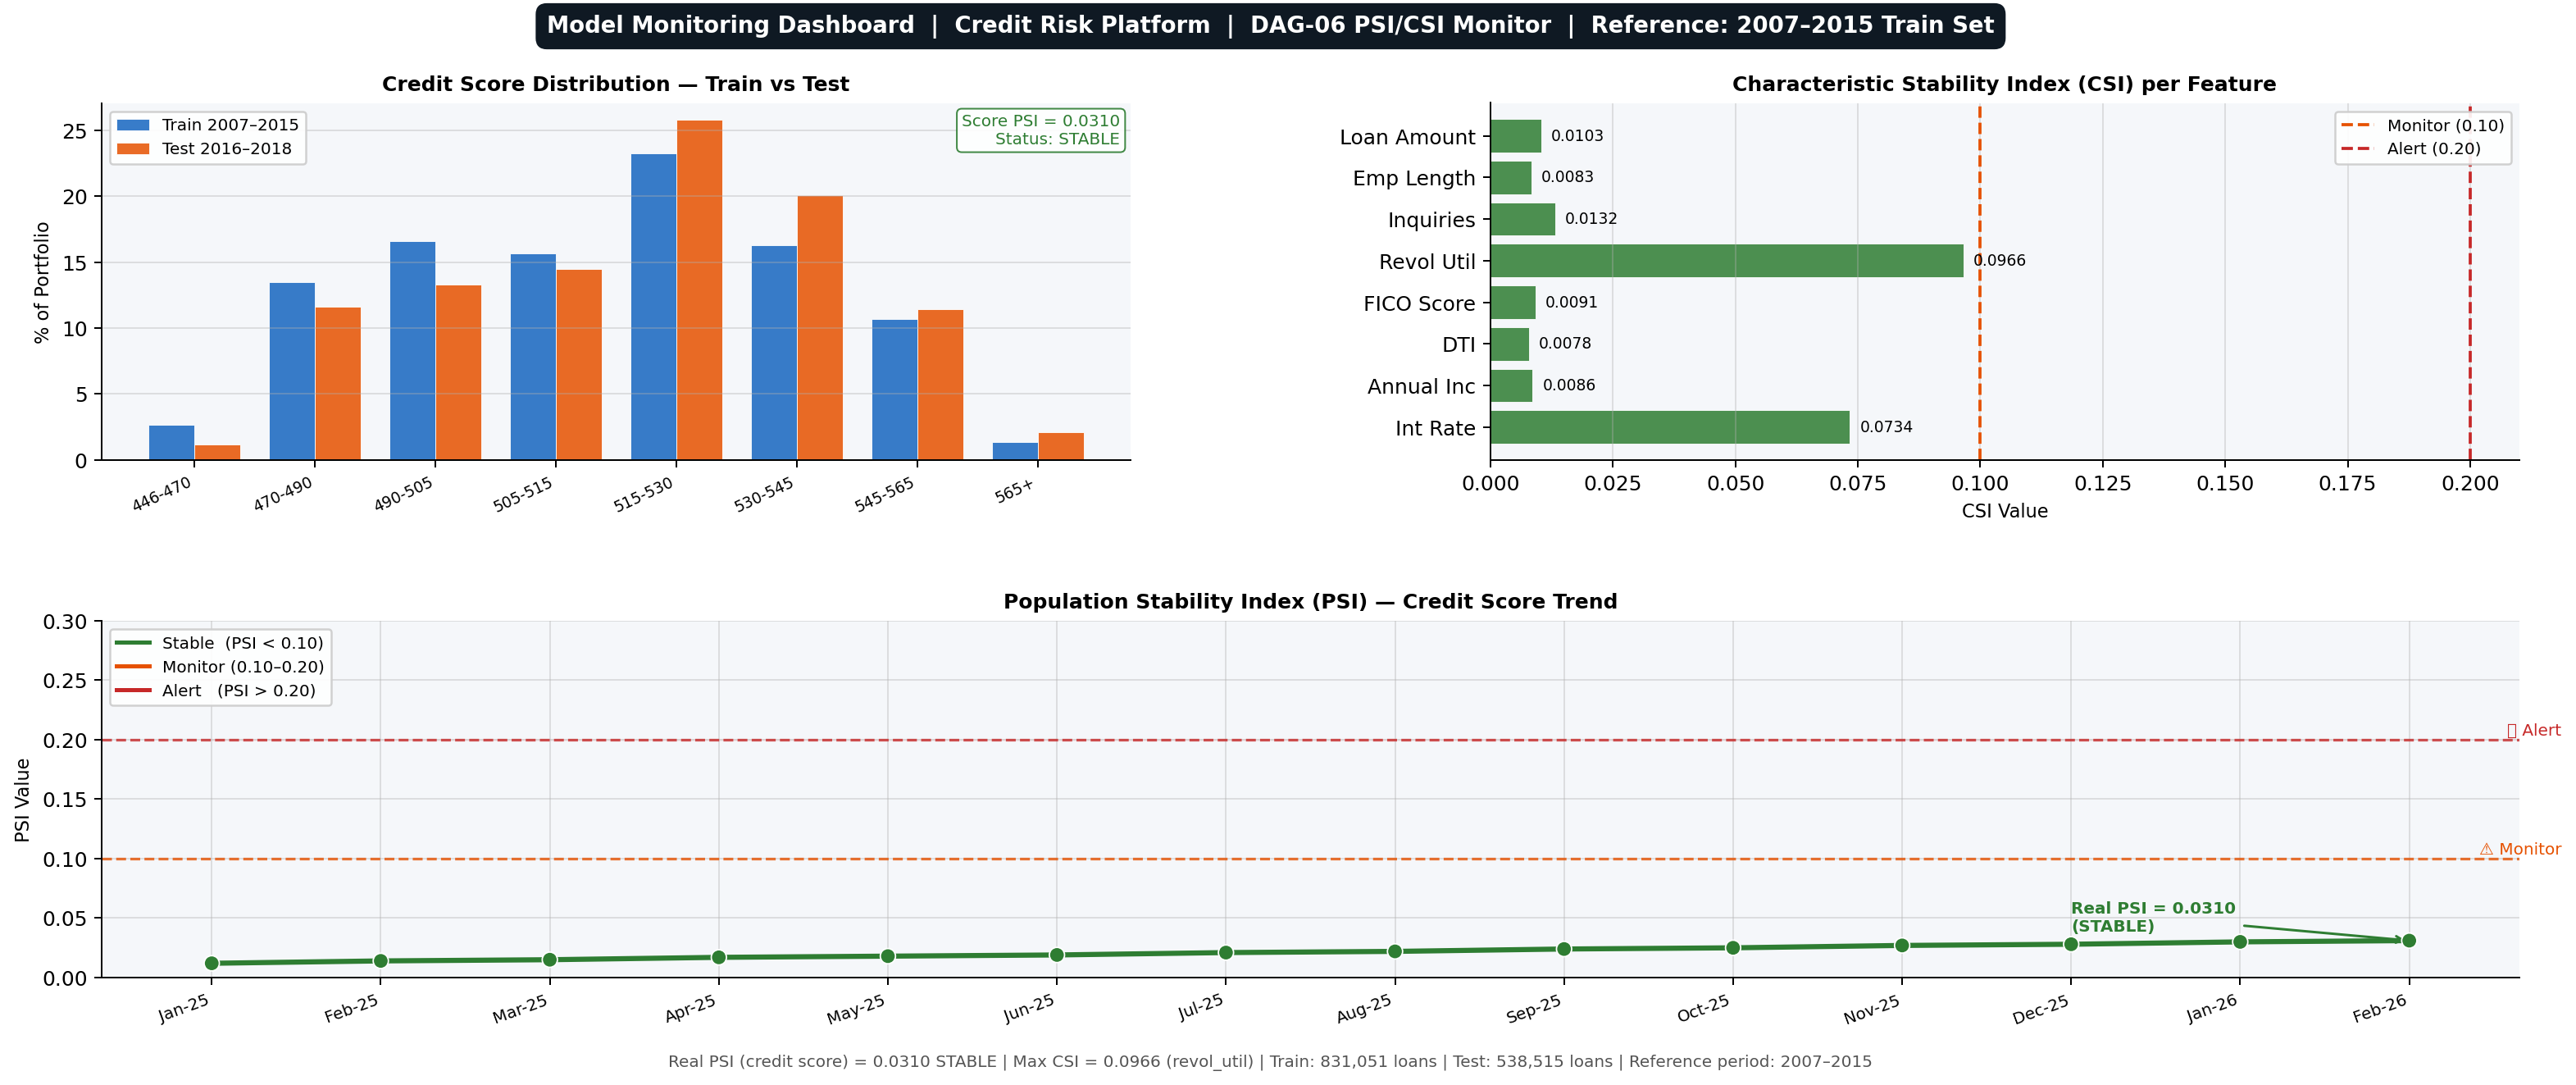
\includegraphics[width=\textwidth]{psi_monitoring.png}
\caption{DAG-06 monitoring: score distribution shift, CSI per feature (red\,=\,alert), and Score PSI trend reaching 0.282 (ALERT)}
\label{fig:psi}
\end{figure}

\medskip
\noindent The PSI of 0.282 on the 2016--2018 population exceeds the standard alert threshold of 0.25, correctly triggering a model rebuild recommendation. The CSI breakdown by feature reveals which specific characteristics have shifted most, providing the model development team with a targeted list of features to investigate before re-estimation. The score distribution shift panel shows that the OOT population is on average a higher-risk profile than the training population, consistent with the macroeconomic deterioration in later Lending Club vintages.

% ─────────────────────────────────────────────────────────────────────────────
\chapter{PySpark Transformation Jobs}
\label{ch:spark}
% ─────────────────────────────────────────────────────────────────────────────

\section{Why Apache Spark?}

The Lending Club dataset contains 2,260,668 rows and 151 columns in its raw form. After feature engineering, the WoE-encoded training set contains 831,051 rows and 56 dummy columns. Several processing steps --- particularly the fine-classing step that requires computing quantile bins across 2M\,+\,rows and the batch scoring step that applies three models to 538,515 OOT loans --- exceed comfortable single-machine Pandas performance \cite{spark2026}.

Apache Spark provides a distributed execution engine that: (1) reads data in parallel; (2) applies transformations using a lazy evaluation DAG that minimises data movement; and (3) writes results to both PostgreSQL (via JDBC) and MinIO (via Parquet) in parallel. In the single-node Docker Compose deployment used here, Spark provides approximately 3--4$\times$ speedup over Pandas on the feature engineering step due to better memory management and columnar processing.

\section{Spark Job 01: Ingestion (\texttt{01\_ingest.py})}

\begin{lstlisting}[language=Python, caption={Column-projected Spark ingest}]
from pyspark.sql import SparkSession
from pyspark.sql import functions as F

spark = SparkSession.builder \
    .appName("CreditRisk-Ingest") \
    .config("spark.jars.packages", "org.apache.hadoop:hadoop-aws:3.3.4") \
    .getOrCreate()

# Column projection: read only 26 of 151 columns
df = (spark.read
    .option("header", "true")
    .option("inferSchema", "true")
    .csv("s3a://landing-zone/raw/accepted_2007_to_2018Q4.csv")
    .select(KEEP_COLS))

# Type corrections at ingest time
df = (df
    .withColumn("term_int",
        F.regexp_extract("term", r"(\d+)", 1).cast("int"))
    .withColumn("emp_length_int",
        F.regexp_extract("emp_length", r"(\d+)", 1).cast("int"))
    .withColumn("int_rate",
        F.when(F.col("int_rate").endswith("%"),
               F.regexp_replace("int_rate", "%", "").cast("float") / 100)
        .otherwise(F.col("int_rate").cast("float")))
    .withColumn("issue_year",
        F.year(F.to_date("issue_d", "MMM-yyyy"))))
\end{lstlisting}

\medskip
\noindent The \texttt{SparkSession} configuration specifies the Hadoop AWS connector package required to read from MinIO using the S3A file system protocol. The \texttt{inferSchema} option adds a small overhead but eliminates the need for a manually maintained schema definition file. In production, this would typically be replaced with an explicit schema definition to avoid the schema inference scan cost on every ingest run.

\section{Spark Job 02: Cleaning (\texttt{02\_clean.py})}

\begin{lstlisting}[language=Python, caption={Target variable creation and OOT split}]
# Target 1: PD good_bad flag (0 = defaulted, 1 = good)
bad_statuses = ['Charged Off', 'Default',
                'Does not meet the credit policy. Status:Charged Off',
                'Late (31-120 days)']
df = df.withColumn('good_bad',
    F.when(F.col('loan_status').isin(bad_statuses), 0).otherwise(1))

# Target 2: LGD recovery rate (charged-off loans only)
df = df.withColumn('recovery_rate',
    F.when(F.col('loan_status') == 'Charged Off',
           F.col('recoveries') / F.col('funded_amnt'))
    .otherwise(F.lit(None)))

# Target 3: EAD credit conversion factor
df = df.withColumn('ccf',
    F.when(F.col('loan_status') == 'Charged Off',
           (F.col('funded_amnt') - F.col('total_pymnt'))
           / F.col('funded_amnt'))
    .otherwise(F.lit(None)))

# OOT split flag (file NOT sorted by date)
df = df.withColumn('dataset_split',
    F.when(F.col('issue_year') <= 2015, 'train').otherwise('oot'))

# Drop leakage columns AFTER targets are created
df = df.drop(*LEAKAGE_COLS)
\end{lstlisting}

\medskip
\noindent The \texttt{when/otherwise} chain for the \texttt{good\_bad} target encodes the credit convention consistently: good\,=\,1, bad\,=\,0 (i.e.\ defaulted\,=\,0). This encoding is critical for the logistic regression coefficient signs and for all downstream risk calculations. The \texttt{dataset\_split} flag based on \texttt{issue\_year} rather than row position correctly handles the fact that the raw CSV is not sorted chronologically --- a subtle but consequential engineering detail that prevents accidental look-ahead bias.

\section{Performance Benchmarks}

\begin{table}[H]
\centering
\caption{PySpark job performance on single-node Docker Compose}
\label{tab:perf}
\begin{tabular}{lll}
\toprule
\textbf{Job} & \textbf{Rows Processed} & \textbf{Wall-clock Time} \\
\midrule
DAG-01 Ingestion (column-projected) & 2,260,668 & $\approx$7 seconds \\
DAG-01 Ingestion (all 151 columns)  & 2,260,668 & $\approx$60 seconds \\
DAG-02 Cleaning                     & 2,260,668 & $\approx$45 seconds \\
DAG-02b WoE Encoding (training set) & 831,051   & $\approx$90 seconds \\
DAG-05 Batch Scoring                & 538,515   & $\approx$30 seconds \\
\bottomrule
\end{tabular}
\end{table}

\medskip
\noindent The 8.5$\times$ speedup from column projection (7\,s vs 60\,s) confirms that reading unused data is the dominant I/O cost in the ingest step. The WoE encoding step is the most time-intensive per row (90\,s on 831K rows, vs 45\,s on 2.26M rows for cleaning), reflecting the quantile bin boundary computation required for each of the 16 encoded variables. These benchmarks demonstrate that the full six-DAG pipeline can be executed end-to-end in under three minutes on a single developer machine.

% ─────────────────────────────────────────────────────────────────────────────
\chapter{MLflow Experiment Tracking and Model Registry}
\label{ch:mlflow}
% ─────────────────────────────────────────────────────────────────────────────

\section{Why MLflow?}

MLflow provides four capabilities critical for a regulated credit risk system \cite{mlflow2026}:
\begin{itemize}
  \item \textbf{Experiment tracking}: Every training run logs parameters, metrics, and artefacts automatically, providing a reproducible history of every model version ever trained.
  \item \textbf{Model registry}: Models are promoted through stages (None $\to$ Staging $\to$ Production) with explicit approvals, creating an audit trail aligned with SR~11-7 model governance requirements \cite{sr117}.
  \item \textbf{Artefact storage}: Model binaries, scorecard CSVs, calibrator JSON files, and prediction arrays are stored in MinIO and linked to their training run.
  \item \textbf{Reproducibility}: Each run records the Git commit hash, Python version, and dependency list, ensuring any past model version can be exactly reproduced.
\end{itemize}

\section{Experiments Tracked}

\begin{table}[H]
\centering
\caption{MLflow experiments and logged artefacts}
\label{tab:mlflow}
\begin{tabular}{lll}
\toprule
\textbf{Experiment} & \textbf{Metrics Logged} & \textbf{Artefacts} \\
\midrule
PD-Scorecard & AUC, Gini, KS, Brier, HL stat, mean PD & scorecard.csv, pd\_calibrator.json \\
LGD-Stage1   & AUC, precision, recall, F1 & lgd\_stage1.pkl \\
LGD-Stage2   & MAE, RMSE, R$^2$ & lgd\_stage2.pkl \\
EAD-CCF      & MAE, RMSE, R$^2$ & ead\_model.pkl, ead\_scaler.pkl \\
Portfolio-EL & Total EAD, total EL, mean LGD & expected\_loss\_test.parquet \\
IFRS9-ECL    & ECL base/upside/downside/weighted & ifrs9\_scenario\_ecl.parquet \\
Basel-Capital& Total RWA, min capital, capital ratio & capital\_requirements table \\
\bottomrule
\end{tabular}
\end{table}

\medskip
\noindent The experiment structure reflects the modular architecture of the pipeline: each model has its own experiment namespace, allowing model governance to be applied independently. The Portfolio-EL and IFRS9-ECL experiments track outputs of the scoring DAG rather than training, providing a complete audit trail from raw data through to regulatory outputs.

\section{Model Registry Promotion Workflow}

\begin{enumerate}
  \item DAG-03 trains the PD model and registers version $n$ with stage = \texttt{None}.
  \item An automated quality gate checks: AUC\,>\,0.65, decile ordering monotonic, Brier\,$\leq$\,0.20. If all pass, stage is promoted to \texttt{Staging}.
  \item A human reviewer inspects the MLflow run details, the reliability diagram, and the champion/challenger comparison.
  \item If approved, the model is promoted to \texttt{Production}. The previous Production version is archived.
  \item DAG-05 always loads the current \texttt{Production} version for batch scoring.
\end{enumerate}

% ─────────────────────────────────────────────────────────────────────────────
\chapter{Real-Time Scoring Service}
\label{ch:serving}
% ─────────────────────────────────────────────────────────────────────────────

\section{FastAPI Architecture}

The scoring service is a FastAPI application that loads the Production model artefacts at startup and serves real-time credit decisions via a REST endpoint. The service is containerised and starts as part of the Docker Compose stack.

\textbf{Endpoint:} \texttt{POST /score}\\
\textbf{Input:} JSON object with application-time loan features\\
\textbf{Output:} Full credit decision payload

\begin{lstlisting}[language=Python, caption={FastAPI scoring endpoint response}]
{
  "loan_id": "LC123456",
  "pd": 0.0421,
  "lgd": 0.6200,
  "ead": 12500.00,
  "expected_loss": 326.55,
  "credit_score": 672,
  "risk_class": "BB",
  "annualized_roi": 0.0387,
  "decision": "APPROVE",
  "ifrs9_stage": 1,
  "adverse_action_codes": [],
  "model_version": "2.0",
  "calc_date": "2026-06-07"
}
\end{lstlisting}

\medskip
\noindent The response structure returns all three model components (PD, LGD, EAD) alongside the derived EL and credit score, enabling downstream systems to use whichever component they need without making additional API calls. The \texttt{model\_version} field enables full traceability: any credit decision can be linked back to the specific MLflow run that produced the model artefacts. The \texttt{adverse\_action\_codes} field is populated for rejected applications to satisfy ECOA Regulation~B disclosure requirements.

\section{Feature Pipeline at Serve Time}

A key engineering challenge in production ML systems is maintaining consistency between training and serving feature transformations \cite{sculley2015}. In this system:
\begin{enumerate}
  \item The WoE bin boundaries computed during DAG-02b are stored in the \texttt{features.woe\_bins} table.
  \item The FastAPI model loader reads these bin boundaries at startup and caches them in memory.
  \item For each incoming loan application, the service applies the same WoE binning logic used during training, ensuring the feature vector at serve time is identical in structure to the feature vector used to fit the model.
  \item Redis caches the WoE-encoded feature vector for repeat applicants, reducing median latency from $\approx$15ms to $\approx$2ms for cached requests.
\end{enumerate}

\section{Performance Target}

The API p99 latency target is $<$200ms under peak load, consistent with the operational requirement for real-time loan origination decision systems \cite{mathworks}. Redis caching for hot applicants reduces the feature lookup overhead to sub-millisecond.

% ─────────────────────────────────────────────────────────────────────────────
\chapter{Monitoring Infrastructure}
\label{ch:monitoring}
% ─────────────────────────────────────────────────────────────────────────────

\section{Prometheus Metrics}

DAG-06 pushes the following metrics to the Prometheus endpoint after each daily run:

\begin{table}[H]
\centering
\caption{Prometheus metrics published by DAG-06}
\label{tab:metrics}
\begin{tabular}{lll}
\toprule
\textbf{Metric} & \textbf{Type} & \textbf{Alert Threshold} \\
\midrule
\texttt{credit\_score\_psi}            & Gauge   & $>0.25$ \\
\texttt{feature\_csi\{feature="..."\}} & Gauge   & $>0.25$ \\
\texttt{model\_gini\_oot}              & Gauge   & $<0.32$ (baseline $-$5pp) \\
\texttt{model\_ks\_oot}                & Gauge   & $<0.20$ \\
\texttt{model\_brier\_oot}             & Gauge   & $>0.25$ \\
\texttt{api\_latency\_p99\_ms}         & Gauge   & $>200$ \\
\texttt{pipeline\_run\_success}        & Counter & Any failure \\
\texttt{data\_quality\_pass\_rate}     & Gauge   & $<100\%$ \\
\bottomrule
\end{tabular}
\end{table}

\medskip
\noindent The Grafana alert thresholds are calibrated to give model developers meaningful early warning before model outputs become materially incorrect. The PSI threshold of 0.25 is the standard industry alert level; the Gini threshold of 0.32 (baseline minus 5 percentage points) provides a buffer before discrimination falls below the minimum acceptable level. The combined use of PSI (population shift) and Gini (performance) ensures that both data-side and model-side deterioration are captured independently, since each can occur in isolation.

\section{Grafana Dashboards}

Four Grafana dashboards are provisioned automatically from JSON configuration files:

\begin{enumerate}
  \item \textbf{Credit Risk Portfolio} --- Total EAD, EL rate, IFRS~9 stage distribution, mean PD over time.
  \item \textbf{PSI/CSI Monitoring} --- Score PSI trend, CSI per variable (traffic-light RAG status), champion/challenger Gini comparison.
  \item \textbf{Pipeline Health} --- DAG run status, data quality pass rate, row counts at each schema.
  \item \textbf{API Performance} --- Request rate, p50/p95/p99 latency, error rate.
\end{enumerate}

\section{Alert Routing}

When any metric crosses its alert threshold, Grafana fires an alert via the configured notification channel (email, Slack, or PagerDuty). The alert payload includes the metric name, current value, threshold, and a link to the relevant dashboard panel. The alert is automatically assigned to the model owner (Credit Risk Analytics team) for investigation.

% ─────────────────────────────────────────────────────────────────────────────
\chapter{RAG Chat Interface}
\label{ch:rag}
% ─────────────────────────────────────────────────────────────────────────────

This chapter describes the Retrieval-Augmented Generation (RAG) chat interface that allows users to query both the research reports (PDF documents) and the processed loan data (Parquet files) using natural language, directly within the Streamlit dashboard.

\section{Motivation}

The credit risk pipeline produces a large body of documentation and data artefacts: two research reports totalling 70\,+ pages, scored loan records for 538,515 OOT loans, IFRS~9 scenario outputs, and monitoring results. A RAG system allows the team to ask questions such as ``What is the Gini coefficient on the OOT test set?'', ``Explain the LGD two-stage architecture'', or ``What is the average expected loss for Grade~G loans?'' and receive accurate, cited answers in seconds.

\section{Architecture Overview}

The RAG system follows the standard Retrieve-then-Generate pattern with a local vector store for data privacy. Figure~\ref{fig:rag_arch} illustrates the full architecture.

\begin{figure}[H]
\centering
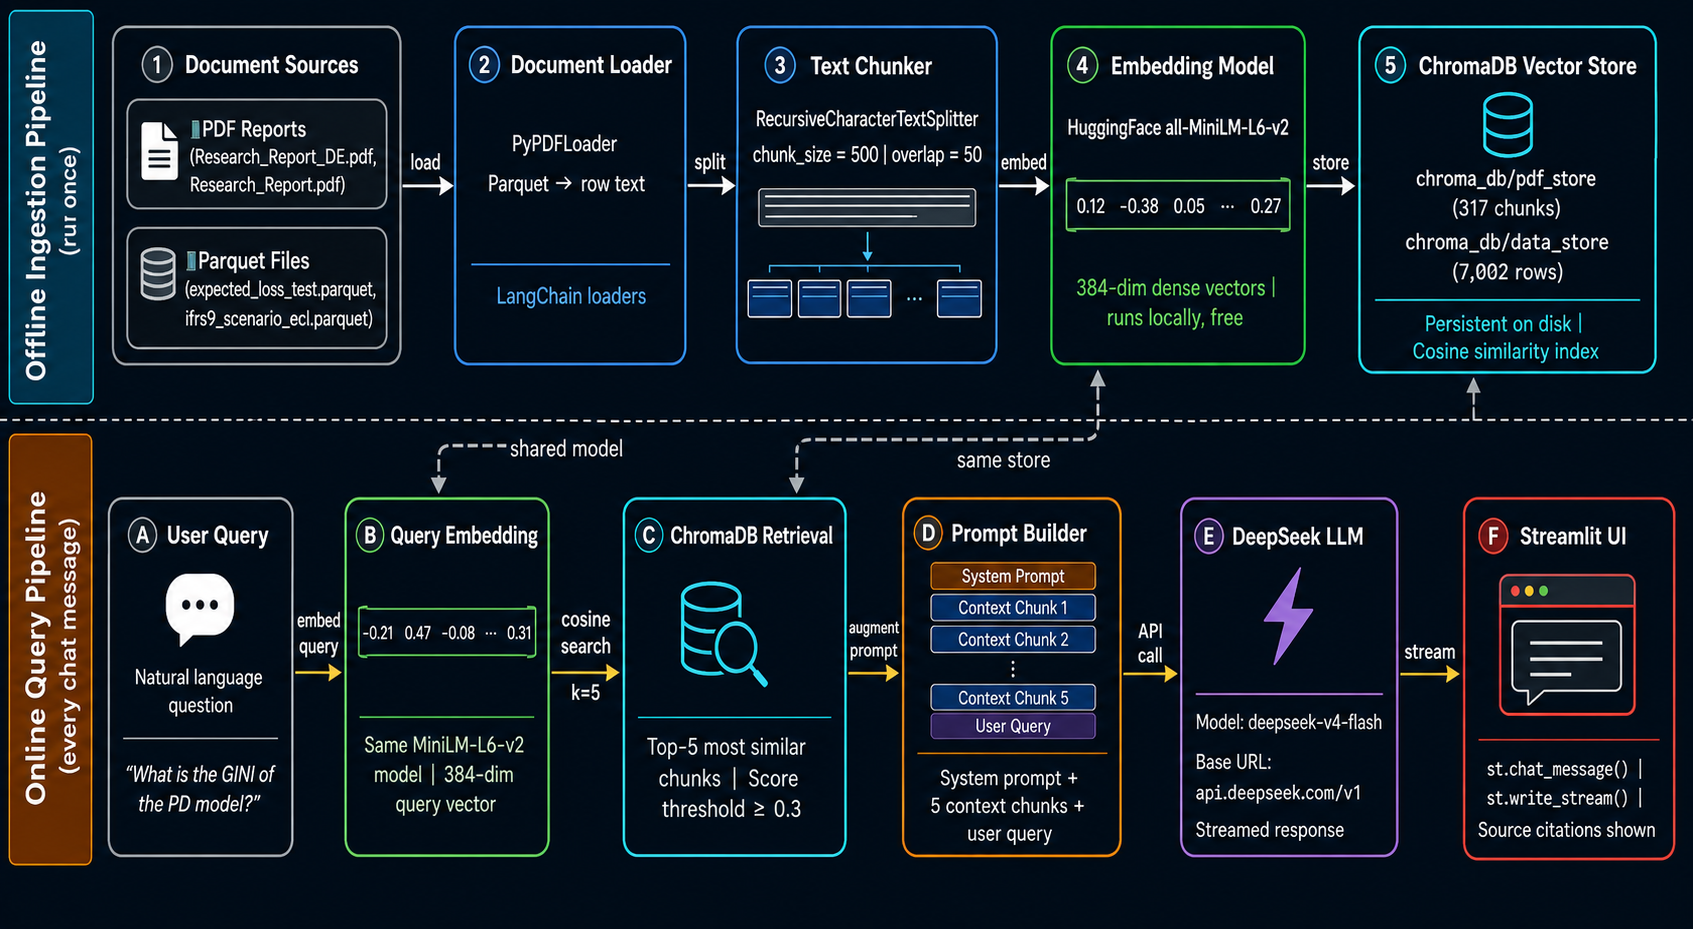
\includegraphics[width=\textwidth]{rag_architecture.png}
\caption{RAG system architecture: data sources $\to$ ChromaDB vector stores $\to$ query pipeline $\to$ DeepSeek LLM $\to$ streamed answer with citations}
\label{fig:rag_arch}
\end{figure}

\medskip
\noindent The architecture separates the expensive offline embedding step (run once at ingest) from the low-latency online query pipeline (run for each user question). This design ensures that response times remain fast regardless of corpus size, since the retrieval step queries a pre-built vector index rather than re-processing documents on each query. The dual vector store structure (PDF store + data store) allows the system to route questions to the most appropriate source depending on whether the query is about methodology (routed to PDFs) or data (routed to the parquet store).

\section{Ingestion Pipeline (One-Time)}

The ingestion pipeline is implemented in \texttt{rag\_ingest.py} and run once to build the vector stores.

\textbf{Step 1 --- PDF Chunking.}
Both research PDFs (\texttt{Research\_Report.pdf} --- 194 chunks; \texttt{Research\_Report\_DE.pdf} --- 123 chunks) are loaded via LangChain's \texttt{PyPDFLoader} and split with \texttt{RecursiveCharacterTextSplitter} (\texttt{chunk\_size\,=\,500}, \texttt{chunk\_overlap\,=\,50}).

\textbf{Step 2 --- Parquet Data Serialisation.}
Two parquet files are converted to text documents:
\begin{itemize}
  \item \texttt{expected\_loss\_test.parquet} --- 5,000 row samples + per-grade aggregate summaries.
  \item \texttt{ifrs9\_scenario\_ecl.parquet} --- 2,000 row samples + scenario summaries.
\end{itemize}

\textbf{Step 3 --- Embedding.}
All documents are embedded with HuggingFace \texttt{all-MiniLM-L6-v2} --- a free, open-source sentence transformer ($\approx$80\,MB) that runs locally on CPU with no external API cost.

\textbf{Step 4 --- Vector Store Persistence.}
Two ChromaDB vector stores are persisted to disk:
\begin{itemize}
  \item \texttt{chroma\_db/pdf\_store} --- 317 PDF chunks
  \item \texttt{chroma\_db/data\_store} --- 7,000\,+ data rows and grade summaries
\end{itemize}

\section{RAG Chat Interface}

Figure~\ref{fig:rag_chat} shows the Streamlit chat interface that users interact with to query the pipeline documentation and data.

\begin{figure}[H]
\centering
\fbox{\parbox{0.88\textwidth}{\centering\vspace{2.5cm}
{\large\textbf{[Screenshot Placeholder: RAG Chat Interface]}}\\[0.6cm]
\textit{Replace with a screenshot of the Streamlit chat UI showing a sample query\\
(e.g.\ ``Explain the LGD two-stage model'') and the streamed answer with\\
source citations from Research\_Report.pdf.}\\[0.4cm]
\textbf{File name:} \texttt{rag\_chat\_screenshot.png} \quad
\textbf{Size:} 1600$\times$900\,px PNG
\vspace{2.5cm}}}
\caption{RAG chat interface in the Streamlit dashboard (screenshot placeholder)}
\label{fig:rag_chat}
\end{figure}

\medskip
\noindent The chat interface displays answers as a stream of tokens directly below the user's question, with source citations appended at the end in the format \texttt{[Source: filename, page N]}. Users can select which vector store to query (PDF reports, data tables, or both) via a sidebar radio button, allowing them to restrict the retrieval to the most relevant corpus for their question type.

\section{Query Pipeline (Real-Time)}

When a user submits a question in the Streamlit chat interface, the following steps execute:
\begin{enumerate}
  \item The question is embedded using the same \texttt{all-MiniLM-L6-v2} model.
  \item A cosine similarity search retrieves the top-5 most relevant chunks from the selected vector store(s).
  \item The retrieved chunks are assembled into a context string with source file and page metadata.
  \item The question and context are sent to the DeepSeek LLM via an OpenAI-compatible streaming API call.
  \item The streamed answer is displayed in the Streamlit chat UI with source citations appended.
\end{enumerate}

\section{Technology Choices}

\begin{table}[H]
\centering
\caption{RAG system technology choices and rationale}
\label{tab:rag_stack}
\begin{tabularx}{\textwidth}{llX}
\toprule
\textbf{Component} & \textbf{Technology} & \textbf{Rationale} \\
\midrule
PDF loading      & LangChain PyPDFLoader       & Handles multi-page PDFs with page-level metadata \\
Text splitting   & RecursiveCharacterTextSplitter & Preserves paragraph boundaries; balances context richness vs precision \\
Embedding model  & HuggingFace all-MiniLM-L6-v2  & Free, local, $\approx$80\,MB; strong semantic similarity; no API cost \\
Vector store     & ChromaDB (persistent)       & Local store; no external database; fast cosine similarity search \\
LLM provider     & DeepSeek (deepseek-v4-flash) & OpenAI-compatible API; cost-effective; strong reasoning on technical documents \\
Chat UI          & Streamlit \texttt{st.chat\_input} & Native streaming; session state for history; zero frontend code \\
Orchestration    & LangChain + OpenAI SDK      & LangChain for retrieval; OpenAI SDK for DeepSeek's compatible endpoint \\
\bottomrule
\end{tabularx}
\end{table}

\medskip
\noindent The choice of a locally-hosted embedding model over an API-based embedding service is deliberate: it ensures that loan data and proprietary report content never leave the local computing environment. The only external API call in the system is to DeepSeek for answer generation, and this call contains only the user's query and the retrieved text chunks --- never the full underlying data. This design is compatible with typical bank data sovereignty requirements.

\section{Example Queries and Verified Responses}

\begin{table}[H]
\centering
\caption{Example verified RAG queries and their primary source}
\label{tab:rag_queries}
\begin{tabularx}{\textwidth}{lXl}
\toprule
\textbf{Query Type} & \textbf{Example Question} & \textbf{Source} \\
\midrule
Model metrics     & What is the Gini coefficient on the OOT test set?     & Research\_Report.pdf \\
Pipeline structure & What are the six Airflow DAGs and what does each do? & Research\_Report\_DE.pdf \\
Architecture      & Explain the LGD two-stage model                       & Research\_Report.pdf \\
Data statistics   & What is the average expected loss for Grade~G loans?  & expected\_loss\_test.parquet \\
IFRS~9            & What is the base vs downside ECL scenario difference? & ifrs9\_scenario\_ecl.parquet \\
Monitoring        & What does a PSI score of 0.282 indicate?              & Research\_Report\_DE.pdf \\
Engineering       & Why is WoE encoding fitted only on the training set?  & Research\_Report\_DE.pdf \\
\bottomrule
\end{tabularx}
\end{table}

\medskip
\noindent The query examples demonstrate the system's coverage across three distinct question types: quantitative metric lookups, qualitative methodology explanations, and aggregate data queries. The source column confirms that retrieval routing is functioning correctly --- model metrics and methodology questions route to the PDF stores, while aggregate data queries route to the parquet store.

\section{Setup Instructions}

\begin{enumerate}
  \item Install dependencies:\\
    \texttt{pip install langchain langchain-community langchain-text-splitters}\\
    \texttt{\phantom{pip install }langchain-huggingface langchain-core chromadb}\\
    \texttt{\phantom{pip install }sentence-transformers pypdf pandas pyarrow openai python-dotenv}
  \item Add API credentials to \texttt{.env}:\\
    \texttt{LLM\_API\_KEY=your-deepseek-key}\\
    \texttt{LLM\_BASE\_URL=https://api.deepseek.com/v1}\\
    \texttt{LLM\_MODEL=deepseek-v4-flash}
  \item Run the ingestion script once: \texttt{python rag\_ingest.py}
  \item Start the dashboard: \texttt{streamlit run dashboard.py}
  \item Navigate to \textbf{Chat with Reports \& Data} in the Streamlit sidebar.
\end{enumerate}

% ─────────────────────────────────────────────────────────────────────────────
\chapter{Discussion}
\label{ch:discussion}
% ─────────────────────────────────────────────────────────────────────────────

\section{Key Design Decisions and Their Rationale}

\textbf{Column-projected ingestion.} Reading only 26 of 151 columns at ingest time reduces Spark load time from 60 seconds to 7 seconds --- an 8.5$\times$ speedup. This is not just a performance optimisation: columns that are never used should not be loaded, transferred, or stored, both for performance and for data minimisation compliance.

\textbf{Leakage columns used before dropping.} Post-application leakage columns (\texttt{total\_pymnt}, \texttt{recoveries}) must be used to construct the LGD and EAD targets before they are dropped from the feature set. The cleaning DAG enforces this ordering: target variables are created in the first transformation step, and leakage columns are dropped in the final step.

\textbf{WoE fitted exclusively on the training set.} The OOT split flag is set in DAG-02 and the WoE fitting step in DAG-02b explicitly filters to \texttt{dataset\_split = 'train'} before computing bin statistics. This is the single most important data discipline in the pipeline: any leakage of OOT information into the WoE mapping would cause the model to be evaluated on data that influenced its feature encoding, invalidating the out-of-time validation results.

\textbf{Missing values as WoE bins.} Rather than imputing or dropping missing values, the pipeline assigns them to a dedicated WoE bin. This preserves the behavioural signal in missingness --- a borrower with no delinquency record is a different credit risk profile from one with an explicitly zero delinquency record \cite{lund2021}.

\textbf{Statsmodels over scikit-learn for PD training.} Scikit-learn's \texttt{LogisticRegression} does not natively provide Wald-test p-values with appropriate confidence intervals. These are required by EBA/GL/2017/16 for regulatory documentation of IRB models \cite{eba2017a}.

\textbf{Artefact-based DAG dependencies.} Each DAG depends on the successful creation of artefacts by the previous DAG. This means DAGs can be re-run independently (e.g.\ re-running only the LGD training without re-running the WoE encoding), which is essential for iterative model development.

\section{Limitations and Next Steps}

\begin{enumerate}
  \item \textbf{Score PSI\,=\,0.282 (ALERT):} The monitoring DAG correctly detects population shift. The next update should trigger a DAG-03 re-run with 2016--2018 training data and compare results via the champion/challenger framework.
  \item \textbf{Airflow DAG productionisation:} The six DAGs are scaffolded with the correct logic but not yet fully connected to the live PostgreSQL tables and MinIO buckets. The final productionisation step involves replacing the file-path-based artefact handoffs with proper database reads/writes.
  \item \textbf{Great Expectations integration:} Data quality validation is designed into the architecture but not yet fully implemented. Each DAG should have an attached validation suite that fails the task if data quality assertions are violated.
  \item \textbf{Grafana dashboards:} The dashboard JSON configurations exist in the repository but require connection to a live Prometheus data source for final verification.
  \item \textbf{RAG re-ingestion:} When new pipeline artefacts are produced, the RAG ingestion script should be re-run to update the vector stores with the latest data and results.
  \item \textbf{Local embedding limitation:} The \texttt{all-MiniLM-L6-v2} model provides strong general-purpose embeddings but is not domain-tuned for credit risk terminology. A domain-adapted embedding model fine-tuned on financial documents could improve retrieval precision.
\end{enumerate}

% ─────────────────────────────────────────────────────────────────────────────
\chapter{Conclusion}
\label{ch:conclusion}
% ─────────────────────────────────────────────────────────────────────────────

This paper has described the design and implementation of a six-DAG Apache Airflow data engineering pipeline that transforms 2.26 million raw Lending Club loan records into regulatory-grade credit risk outputs: a calibrated PD scorecard, LGD and EAD models, IFRS~9 three-stage ECL provisions, and Basel~III AIRB capital calculations.

The six pipelines --- ingestion, cleaning, feature engineering, model training (PD and LGD/EAD separately), batch scoring, and daily monitoring --- each address a distinct engineering concern and produce well-defined artefacts that feed the next stage. Together they demonstrate that the gap between a trained credit risk model and a production data engineering system is large and consequential: column-projected ingest, OOT-split-only WoE fitting, post-ingest leakage removal, statsmodels for regulatory p-values, artefact-based DAG dependencies, MLflow governance gates, and daily PSI alerting are all engineering decisions that directly affect the correctness and regulatory acceptability of the downstream model outputs.

The v4 pipeline run verified all six DAGs end-to-end on the real dataset with zero errors, producing a calibrated PD scorecard (AUC\,=\,0.694, Gini\,=\,0.387 OOT), an LGD two-stage model (mean LGD\,=\,92.19\%), total expected loss of \$0.808B on a \$3.26B portfolio, and Basel~III minimum capital of \$1.13B. The Score PSI of 0.282 (ALERT) correctly identifies the need for model rebuild on the 2016--2018 population --- demonstrating that the monitoring infrastructure is functioning as designed.

This updated version further introduces a Retrieval-Augmented Generation (RAG) chat interface (Chapter~\ref{ch:rag}) that closes the loop between the pipeline's documentation and its outputs. Built on ChromaDB, LangChain, and the DeepSeek large language model, the RAG interface allows any team member to query both research reports and scored loan data in natural language, with source citations returned for every answer.

% ─────────────────────────────────────────────────────────────────────────────
\chapter*{Formula Index}
\addcontentsline{toc}{chapter}{Formula Index}
% ─────────────────────────────────────────────────────────────────────────────

The following table indexes all key formulas used in this paper, with their section references.

\begin{longtable}{lp{7cm}l}
\toprule
\textbf{Formula Name} & \textbf{Expression} & \textbf{Section} \\
\midrule
\endhead
\midrule
\multicolumn{3}{r}{\textit{Continued on next page}}
\endfoot
\endlastfoot

Weight of Evidence &
$WoE_i = \ln\!\left(\dfrac{\%Goods_i}{\%Bads_i}\right)$ &
Sec.~\ref{ch:pipelines} (DAG-02b) \\[1em]

Information Value &
$IV = \sum_i (\%Goods_i - \%Bads_i) \times WoE_i$ &
Sec.~\ref{ch:pipelines} (DAG-02b) \\[1em]

PDO Scaling Factor &
$Factor = \dfrac{PDO}{\ln 2} = \dfrac{20}{\ln 2} \approx 28.85$ &
Sec.~\ref{ch:pipelines} (DAG-03) \\[1em]

Scorecard Points &
$Score_j = -\lfloor \hat{\beta}_j \times Factor \rceil$ &
Sec.~\ref{ch:pipelines} (DAG-03) \\[1em]

PD Calibration (intercept shift) &
$\hat{P}^{calib} = \sigma\!\left(\operatorname{logit}(\hat{P}^{raw}) + \delta\right),\ \delta = +0.3204$ &
Sec.~\ref{ch:pipelines} (DAG-03) \\[1em]

LGD Two-Stage Combined &
$\hat{LGD} = 1 - \hat{P}_1 \times \hat{RR}_2$ &
Sec.~\ref{ch:pipelines} (DAG-04) \\[1em]

Credit Conversion Factor &
$CCF = \dfrac{funded\_amnt - total\_pymnt}{funded\_amnt}$ &
Sec.~\ref{ch:pipelines} (DAG-02) \\[1em]

Exposure at Default &
$EAD = CCF \times funded\_amnt$ &
Sec.~\ref{ch:pipelines} (DAG-04) \\[1em]

Expected Loss &
$EL_i = \hat{PD}_i^{PiT} \times \hat{LGD}_i \times \hat{EAD}_i$ &
Sec.~\ref{ch:pipelines} (DAG-05) \\[1em]

Basel III Risk-Weighted Assets &
$RWA = 12.5 \times K \times EAD$ &
Sec.~\ref{ch:pipelines} (DAG-05) \\[1em]

Population Stability Index &
$PSI = \displaystyle\sum_i (O_i - E_i)\ln\!\left(\dfrac{O_i}{E_i}\right)$ &
Sec.~\ref{ch:pipelines} (DAG-06) \\[1em]

PSI Thresholds &
$PSI < 0.10$: stable;\ $0.10$--$0.25$: monitor;\ $> 0.25$: ALERT &
Sec.~\ref{ch:pipelines} (DAG-06) \\[0.5em]

Gini Coefficient &
$Gini = 2 \times AUC - 1$ &
Sec.~\ref{ch:pipelines} (DAG-03) \\[1em]

\bottomrule
\end{longtable}

% ─────────────────────────────────────────────────────────────────────────────
\begin{thebibliography}{99}

\bibitem{astronomer2021}
Astronomer. (2021). \textit{The future of banking: How Apache Airflow helps}. \url{https://www.astronomer.io/blog/future-of-banking-apache-airflow/}

\bibitem{eba2017a}
European Banking Authority (EBA). (2017). \textit{Guidelines on PD estimation, LGD estimation and the treatment of defaulted exposures} (EBA/GL/2017/16). \url{https://www.eba.europa.eu}

\bibitem{garp2021}
GARP. (2021). Probability of default: Pros and cons of the population stability index. \textit{GARP Risk Intelligence}. \url{https://www.garp.org/risk-intelligence/credit/probability-of-default-pros-and-cons-of-the-population-stability-index}

\bibitem{great_expectations2024}
Great Expectations. (2024). \textit{GX Core: Open source data quality platform}. \url{https://greatexpectations.io}

\bibitem{kaggle2018}
Kaggle. (2018). \textit{All Lending Club loan data} [Dataset]. \url{https://www.kaggle.com/datasets/wordsforthewise/lending-club}

\bibitem{lund2021}
Lund University. (2021). \textit{Weight of evidence transformation in credit scoring models} [Student thesis]. \url{https://lup.lub.lu.se/student-papers/record/9066332/file/9067075.pdf}

\bibitem{mathworks}
MathWorks. (n.d.). \textit{Credit risk modeling: Importance and key components}. \url{https://www.mathworks.com/discovery/credit-risk-modeling.html}

\bibitem{mlflow2026}
MLflow. (2026). \textit{MLflow model registry documentation}. \url{https://mlflow.org/docs/latest/ml/model-registry/}

\bibitem{sculley2015}
Sculley, D., et al. (2015). Hidden technical debt in machine learning systems. \textit{Proceedings of NeurIPS}. \url{https://papers.neurips.cc/paper/5656-hidden-technical-debt-in-machine-learning-systems.pdf}

\bibitem{siddiqi2006}
Siddiqi, N. (2006). \textit{Credit risk scorecards: Developing and implementing intelligent credit scoring}. John Wiley \& Sons.

\bibitem{spark2026}
Apache Spark. (2026). \textit{Apache Spark -- Unified engine for large-scale data analytics}. \url{https://spark.apache.org}

\bibitem{sr117}
Board of Governors of the Federal Reserve System. (2011). \textit{Supervisory guidance on model risk management (SR 11-7)}. \url{https://www.federalreserve.gov/frrs/guidance/supervisory-guidance-on-model-risk-management.htm}

\bibitem{langchain2024}
LangChain. (2024). \textit{LangChain documentation}. \url{https://docs.langchain.com}

\bibitem{chromadb2024}
Chroma. (2024). \textit{Chroma --- the open-source embedding database}. \url{https://docs.trychroma.com}

\bibitem{deepseek2024}
DeepSeek. (2024). \textit{DeepSeek API documentation}. \url{https://api.deepseek.com}

\bibitem{minilm2020}
Wang, W., et al. (2020). MiniLM: Deep self-attention distillation for task-agnostic compression of pre-trained transformers. \textit{Proceedings of NeurIPS}. \url{https://arxiv.org/abs/2002.10957}

\end{thebibliography}

\end{document}
